%%%%%%%%%%%%%%%%%%%%%%%%%%%%%%%%%%%%%%%%%%%%%%%%%%%%%%%%%%%%%%%%%%%%%%%%%%%%%%%%
%  Zawartość: Główny plik szablonu pracy dyplomowej (magisterskiej/inżynierskiej). 
%  Opracował: Tomasz Kubik <tomasz.kubik@pwr.edu.pl>
%  Data: styczeń 2023
%  Wersja: 0.9
%  Wymagania: kompilator pdflatex
%%%%%%%%%%%%%%%%%%%%%%%%%%%%%%%%%%%%%%%%%%%%%%%%%%%%%%%%%%%%%%%%%%%%%%%%%%%%%%%%

\documentclass[a4paper,onecolumn,oneside,12pt,extrafontsizes]{memoir}
%  W celu przygotowania wydruku do archiwum można:
%  a) przygotować pdf, w którym dwie strony zostaną wstawione na jedną fizyczną stronę i taki dokument wydrukować dwustronnie (podejście zalecane)
%
%   Taki dokument można przygotować poprzez
%   - wydruk z Adobe Acrobat Reader z opcją "Wiele" - sekcja "Rozmiar i obsługa stron"
%   - wykorzystanie narzędzi psutils
%
%      Windows (zakładając, że w dystrybucji MiKTeX jest pakiet miktex-psutils-bin-x64-2.9):
%        "c:\Program Files\MiKTeX 2.9\miktex\bin\x64\pdf2ps.exe" Dyplom.pdf Dyplom.ps
%        "c:\Program Files\MiKTeX 2.9\miktex\bin\x64\psnup.exe" -2 Dyplom.ps Dyplom2.ps
%        "c:\Program Files\MiKTeX 2.9\miktex\bin\x64\ps2pdf.exe" Dyplom2.ps Dyplom2.pdf
%        Del Dyplom2.ps Dyplom.ps
%
%     Linux:
%        pdf2ps Dyplom.pdf - | psnup -2 | ps2pdf - Dyplom2.pdf
%
%  b) przekomplilować dokument zmniejszając czcionkę (podejście niezalecane, bo zmienia formatowanie dokumentu)
%
%    Do tego wystarczy posłużyć się poniższymi komendami (zamiast documentclass z pierwszej linijki):
%   \documentclass[a4paper,onecolumn,twoside,10pt]{memoir} 
%   \renewcommand{\normalsize}{\fontsize{8pt}{10pt}\selectfont}

%\usepackage[cp1250]{inputenc} % Proszę zostawić, jeśli kodowanie edytowanych plików to cp1250 
\usepackage[utf8]{inputenc} % Proszę użyć zamiast powyższego, jeśli kodowanie edytowanych plików to UTF8
\usepackage[T1]{fontenc}
\usepackage[english,polish]{babel} % Tutaj ważna jest kolejność atrybutów (dla pracy po polsku polish powinno być na końcu)
%\DisemulatePackage{setspace}
\usepackage{setspace}
\usepackage{color,calc}
%\usepackage{soul} % pakiet z komendami do podkreślania, przekreślania, podświetlania tekstu (raczej niepotrzebny)
\usepackage{ebgaramond} % pakiet z czcionkami garamond, potrzebny tylko do strony tytułowej, musi wystąpić przed pakietem tgtermes
\usepackage{float}

%% Aby uzyskać polskie literki w pdfie (a nie zlepki) korzystamy z pakietu czcionek tgterms. 
%% W pakiecie tym są zdefiniowane klony czcionek Times o kształtach: normalny, pogrubiony, italic, italic pogrubiony.
%% W pakiecie tym brakuje czcionki o kształcie: slanted (podobny do italic). 
%% Jeśli w dokumencie gdzieś zostanie zastosowana czcionka slanted (np. po użyciu komendy \textsl{}), to
%% latex dokona podstawienia na czcionkę standardową i zgłosi to w ostrzeżeniu (warningu).
%% Ponadto tgtermes to czcionka do tekstu. Wszelkie matematyczne wzory będą sformatowane domyślną czcionką do wzorów.
%% Jeśli wzory mają być sformatowane z wykorzystaniem innych czcionek, trzeba to jawnie zadeklarować.

%% Po zainstalowaniu pakietu tgtermes może będzie trzeba zauktualizować informacje 
%% o dostępnych fontach oraz mapy. Można to zrobić z konsoli (jako administrator)
%% initexmf --admin --update-fndb
%% initexmf --admin --mkmaps

\usepackage{tgtermes}   
\renewcommand*\ttdefault{txtt}


%%%%%%%%%%%%%%%%%%%%%%%%%%%%%%%%%%%%%%%%%%%%%%%%%%%%%%%%%%%%%%%%%%%%%%%%%%%%%%%%
%% Ustawienia odpowiedzialne za sposób łamania dokumentu
%% i ułożenie elementów pływających
%%%%%%%%%%%%%%%%%%%%%%%%%%%%%%%%%%%%%%%%%%%%%%%%%%%%%%%%%%%%%%%%%%%%%%%%%%%%%%%%
%\hyphenpenalty=10000		% nie dziel wyrazów zbyt często
\clubpenalty=10000      % kara za sierotki
\widowpenalty=10000     % nie pozostawiaj wdów
%\brokenpenalty=10000		% nie dziel wyrazów między stronami - trzeba było wyłączyć, bo nie łamały się linie w lstlisting
%\exhyphenpenalty=999999		% nie dziel słów z myślnikiem - trzeba było wyłączyć, bo nie łamały się linie w lstlisting
\righthyphenmin=3			  % dziel minimum 3 litery

%\tolerance=4500
%\pretolerance=250
%\hfuzz=1.5pt
%\hbadness=1450

\renewcommand{\topfraction}{0.95}
\renewcommand{\bottomfraction}{0.95}
\renewcommand{\textfraction}{0.05}
\renewcommand{\floatpagefraction}{0.35}

%%%%%%%%%%%%%%%%%%%%%%%%%%%%%%%%%%%%%%%%%%%%%%%%%%%%%%%%%%%%%%%%%%%%%%%%%%%%%%%%
%%  Ustawienia rozmiarów: tekstu, nagłówka i stopki, marginesów
%%  dla dokumentów klasy memoir 
%%%%%%%%%%%%%%%%%%%%%%%%%%%%%%%%%%%%%%%%%%%%%%%%%%%%%%%%%%%%%%%%%%%%%%%%%%%%%%%%
\setlength{\headsep}{10pt} 
\setlength{\headheight}{13.6pt} % wartość baselineskip dla czcionki 11pt tj. \small wynosi 13.6pt
\setlength{\footskip}{\headsep+\headheight}
\setlength{\uppermargin}{\headheight+\headsep+1cm}
\setlength{\textheight}{\paperheight-\uppermargin-\footskip-1.5cm}
\setlength{\textwidth}{\paperwidth-5cm}
\setlength{\spinemargin}{2.5cm}
\setlength{\foremargin}{2.5cm}
\setlength{\marginparsep}{2mm}
\setlength{\marginparwidth}{2.3mm}
%\settrimmedsize{297mm}{210mm}{*}
%\settrims{0mm}{0mm}	
\checkandfixthelayout[fixed] % konieczne, aby się dobrze wszystko poustawiało
%%%%%%%%%%%%%%%%%%%%%%%%%%%%%%%%%%%%%%%%%%%%%%%%%%%%%%%%%%%%%%%%%%%%%%%%%%%%%%%%
%%  Ustawienia odległości linii, wcięć, odstępów
%%%%%%%%%%%%%%%%%%%%%%%%%%%%%%%%%%%%%%%%%%%%%%%%%%%%%%%%%%%%%%%%%%%%%%%%%%%%%%%%
\linespread{1}
%\linespread{1.241}
\setlength{\parindent}{14.5pt}


\usepackage{multicol} % pakiet umożliwiający stworzenie wielokolumnowego tekstu
%%%%%%%%%%%%%%%%%%%%%%%%%%%%%%%%%%%%%%%%%%%%%%%%%%%%%%%%%%%%%%%%%%%%%%%%%%%%%%%%
%% Pakiety do formatowania tabel
%%%%%%%%%%%%%%%%%%%%%%%%%%%%%%%%%%%%%%%%%%%%%%%%%%%%%%%%%%%%%%%%%%%%%%%%%%%%%%%%
\usepackage{tabularx}
% Proszę używać tylko tabularx. Innych pakietów proszę nie stosować !!!
% Dokument na pewno da się zredagować bez ich użycia.
%\usepackage{longtable}
%\usepackage{ltxtable}
%\usepackage{tabulary}

%%%%%%%%%%%%%%%%%%%%%%%%%%%%%%%%%%%%%%%%%%%%%%%%%%%%%%%%%%%%%%%%%%%%%%%%%%%%%%%%
%% Pakiet do wstawiania fragmentów kodu
%%%%%%%%%%%%%%%%%%%%%%%%%%%%%%%%%%%%%%%%%%%%%%%%%%%%%%%%%%%%%%%%%%%%%%%%%%%%%%%%
\usepackage{listings} 
\usepackage{xpatch}
\makeatletter
\xpatchcmd\l@lstlisting{1.5em}{0em}{}{}
\makeatother
% Pakiet dostarcza otoczenia lstlisting. Jest ono wysoce konfigurowalne. 
% Konfigurować można indywidualnie każdy z listingów lub globalnie, w poleceniu \lstset{}.

% Zalecane jest, by kod źródłowy był wyprowadzany z użyciem czcionki maszynowej \ttfamily
% Ponieważ kod źródłowy, nawet po obcięciu do interesujących fragmentów, bywa obszerny, należy zmniejszyć czcionkę.
% Zalecane jest \small (dla krótkich fragmentów) oraz \footnotesize (dla dłuższych fragmentów).

% Ponadto podczas konfiguracji można zadeklarować sposób numerowania linii. Numerowanie linii zalecane jest jednak 
% tylko w przypadkach, gdy w redagowanym tekście znajdują się jakieś odwołania do konkretnych linii.
% Jeśli takich odwołań nie ma, numerowanie linii jest zbędne. Proszę wtedy go nie stosować.
% Przy włączaniu numerowania linii należy zwrócić uwagę na to, gdzie pojawią się te numery.
% Bez zmiany dodatkowych parametrów pojawiają się one na marginesie strony (co jest niepożądane).

\lstset{
  basicstyle=\small\ttfamily, % lub basicstyle=\footnotesize\ttfamily
  %%columns=fullflexible,
	%%showstringspaces=false,
	%%showspaces=false,
  breaklines=true,
  postbreak=\mbox{\textcolor{red}{$\hookrightarrow$}\space}, 
  %%numbers=left,  % ta i poniższe linie dotyczą ustawienia numerowania i sposobu jego wyprowadzania
  %%firstnumber=1, 
  %%numberfirstline=true, 
	%%xleftmargin=17pt,
  %%framexleftmargin=17pt,
  %%framexrightmargin=5pt,
  %%framexbottommargin=4pt,
	belowskip=.5\baselineskip,
	literate={\_}{{\_\allowbreak}}1 % ta deklaracja przydaje się, jeśli na listingu mają być łamane nazwy zawierające podkreślniki
}

% Jeśli edytowany plik nie jest w kodowaniu cp1250, to jest problem z polskimi znakami występującymi we wstawianym kodzie.
% Dlatego podczas pracy na plikach w kodowaniu UTF8 trzeba zadeklarować mapowanie jak niżej (wystarczy odmarkować).
% Niestety, jak się zastosuje to mapowanie mogą pojawić się problemy z podświetlaniem składni (patrz dalej).
\lstset{literate=%-
{ą}{{\k{a}}}1 {ć}{{\'c}}1 {ę}{{\k{e}}}1 {ł}{{\l{}}}1 {ń}{{\'n}}1 {ó}{{\'o}}1 {ś}{{\'s}}1 {ż}{{\.z}}1 {ź}{{\'z}}1 {Ą}{{\k{A}}}1 {Ć}{{\'C}}1 {Ę}{{\k{E}}}1 {Ł}{{\L{}}}1 {Ń}{{\'N}}1 {Ó}{{\'O}}1 {Ś}{{\'S}}1 {Ż}{{\.Z}}1 {Ź}{{\'Z}}1 
    {Ö}{{\"O}}1
    {Ä}{{\"A}}1
    {Ü}{{\"U}}1
    {ß}{{\ss}}1
    {ü}{{\"u}}1
    {ä}{{\"a}}1
    {ö}{{\"o}}1
    {~}{{\textasciitilde}}1
		{—}{{{\textemdash} }}1
}%{\ \ }{{\ }}1}


%% lstlisting pozwala na ostylowania podświetlania składni wybranych języków.
%% Działa to na zasadzie zdefiniowania słów kluczowych oraz sposobu ich wyświetlania.
%% Ponieważ jest to prosty mechanizm, czasem trudno osiągnąć takie efekty, jakie dają narzędzia IDE. 
%% Jednak w większości przypadku osiągane rezutlaty są zadowalające.


%% lstlisting obsługuje domyślnie kilka najpopularniejszych języków.
%%\lstloadlanguages{% Check Dokumentation for further languages ...
%%C,
%%C++,
%%csh,
%%Java
%%}
%% Inne języki muszą być dodefiniowane. Poniżej podano przykłady definicji języków i styli.

\definecolor{lightgray}{rgb}{.9,.9,.9}
\definecolor{darkgray}{rgb}{.4,.4,.4}
\definecolor{purple}{rgb}{0.65, 0.12, 0.82}
\definecolor{javared}{rgb}{0.6,0,0} % for strings
\definecolor{javagreen}{rgb}{0.25,0.5,0.35} % comments
\definecolor{javapurple}{rgb}{0.5,0,0.35} % keywords
\definecolor{javadocblue}{rgb}{0.25,0.35,0.75} % javadoc
 
\lstdefinelanguage{JavaScript}{ 
	keywords={typeof, new, true, false, catch, function, return, null, catch, switch, var, if, in, while, do, else, case, break},
	keywordstyle=\color{blue}\bfseries,
	ndkeywords={class, export, boolean, throw, implements, import, this},
	ndkeywordstyle=\color{darkgray}\bfseries,
	identifierstyle=\color{black},
	sensitive=false,
	comment=[l]{//},
	morecomment=[s]{/*}{*/},
	commentstyle=\color{purple}\ttfamily,
	stringstyle=\color{red}\ttfamily,
	morestring=[b]',
	morestring=[b]"
}
\lstdefinestyle{JavaScriptStyle}{
	language=JavaScript,
	commentstyle=\color{javagreen}, % niestety, jeśli w linii komentarza pojawią się słowa kluczowe, to zostaną pokolorowane
	backgroundcolor=,%\color{lightgray}, % można ustwić kolor tła, ale jest to niezalecane
	extendedchars=true,
	basicstyle=\footnotesize\ttfamily,
	showstringspaces=false,
	showspaces=false,
	numbers=none,%left,
	numberstyle=\footnotesize,
	numbersep=9pt,
	tabsize=2,
	breaklines=true,
	showtabs=false,
	captionpos=t
}

\lstdefinestyle{JavaStyle}{
basicstyle=\footnotesize\ttfamily,
keywordstyle=\color{javapurple}\bfseries,
stringstyle=\color{javared},
commentstyle=\color{javagreen},
morecomment=[s][\color{javadocblue}]{/**}{*/},
numbers=none,%left,
numberstyle=\tiny\color{black},
stepnumber=2,
numbersep=10pt,
tabsize=2,
showspaces=false,
showstringspaces=false,
captionpos=t
}

\definecolor{pblue}{rgb}{0.13,0.13,1}
\definecolor{pgreen}{rgb}{0,0.5,0}
\definecolor{pred}{rgb}{0.9,0,0}
\definecolor{pgrey}{rgb}{0.46,0.45,0.48}
\definecolor{dark-grey}{rgb}{0.4,0.4,0.4}
% styl json
\newcommand\JSONnumbervaluestyle{\color{blue}}
\newcommand\JSONstringvaluestyle{\color{red}}

\newif\ifcolonfoundonthisline

\makeatletter

\lstdefinestyle{json-style}  
{
	showstringspaces    = false,
	keywords            = {false,true},
	alsoletter          = 0123456789.,
	morestring          = [s]{"}{"},
	stringstyle         = \ifcolonfoundonthisline\JSONstringvaluestyle\fi,
	MoreSelectCharTable =%
	\lst@DefSaveDef{`:}\colon@json{\processColon@json},
	basicstyle          = \footnotesize\ttfamily,
	keywordstyle        = \ttfamily\bfseries,
	numbers				= left, % zakomentować, jeśli numeracja linii jest niepotrzebna
	numberstyle={\footnotesize\ttfamily\color{dark-grey}},
	xleftmargin			= 2em % zakomentować, jeśli numeracja linii jest niepotrzebna
}

\newcommand\processColon@json{%
	\colon@json%
	\ifnum\lst@mode=\lst@Pmode%
	\global\colonfoundonthislinetrue%
	\fi
}

\lst@AddToHook{Output}{%
	\ifcolonfoundonthisline%
	\ifnum\lst@mode=\lst@Pmode%
	\def\lst@thestyle{\JSONnumbervaluestyle}%
	\fi
	\fi
	\lsthk@DetectKeywords% 
}

\lst@AddToHook{EOL}%
{\global\colonfoundonthislinefalse}

\makeatother


\newcommand\YAMLcolonstyle{\color{red}\mdseries}
\newcommand\YAMLkeystyle{\color{black}\bfseries}
\newcommand\YAMLvaluestyle{\color{blue}\mdseries}

\makeatletter

% here is a macro expanding to the name of the language
% (handy if you decide to change it further down the road)
\newcommand\language@yaml{yaml}

\expandafter\expandafter\expandafter\lstdefinelanguage
\expandafter{\language@yaml}
{
  keywords={true,false,null,y,n},
  keywordstyle=\color{darkgray}\bfseries,
  basicstyle=\YAMLkeystyle\ttfamily\footnotesize,                                 % assuming a key comes first
  sensitive=false,
  comment=[l]{\#},
  morecomment=[s]{/*}{*/},
  commentstyle=\color{purple}\ttfamily,
  stringstyle=\YAMLvaluestyle\ttfamily,
  moredelim=[l][\color{orange}]{\&},
  moredelim=[l][\color{magenta}]{*},
  moredelim=**[il][\YAMLcolonstyle{:}\YAMLvaluestyle]{:},   % switch to value style at :
  morestring=[b]',
  morestring=[b]",
  literate =    {---}{{\ProcessThreeDashes}}3
                {>}{{\textcolor{red}\textgreater}}1     
                {|}{{\textcolor{red}\textbar}}1 
                {\ -\ }{{\mdseries\ -\ }}3,
}

% switch to key style at EOL
\lst@AddToHook{EveryLine}{\ifx\lst@language\language@yaml\YAMLkeystyle\fi}
\makeatother

\newcommand\ProcessThreeDashes{\llap{\color{cyan}\mdseries-{-}-}}

\makeatletter

\lstdefinelanguage{docker}{
	keywords={FROM, RUN, COPY, ADD, ENTRYPOINT, CMD,  ENV, ARG, WORKDIR, EXPOSE, LABEL, USER, VOLUME, STOPSIGNAL, ONBUILD, MAINTAINER, HEALTHCHECK},
  keywordstyle=\color{black}\bfseries,
  identifierstyle=\color{blue},
  sensitive=true,
  comment=[l]{\#},
  commentstyle=\color{purple}\ttfamily,
  inputencoding=utf8,
  extendedchars=true,
	basicstyle=\color{blue}\ttfamily\footnotesize
}

\makeatother


%%\definecolor{red}{rgb}{0.6,0,0} % for strings
%%\definecolor{blue}{rgb}{0,0,0.6}
%%\definecolor{green}{rgb}{0,0.8,0}
%%\definecolor{cyan}{rgb}{0.0,0.6,0.6}
%%
%%\lstdefinestyle{sqlstyle}{
%%language=SQL,
%%basicstyle=\footnotesize\ttfamily, 
%%numbers=left, 
%%numberstyle=\tiny, 
%%numbersep=5pt, 
%%tabsize=2, 
%%extendedchars=true, 
%%breaklines=true, 
%%showspaces=false, 
%%showtabs=true, 
%%xleftmargin=17pt,
%%framexleftmargin=17pt,
%%framexrightmargin=5pt,
%%framexbottommargin=4pt,
%%keywordstyle=\color{blue}, 
%%commentstyle=\color{green}, 
%%stringstyle=\color{red}, 
%%}
%%
%%\lstdefinestyle{sharpcstyle}{
%%language=[Sharp]C,
%%basicstyle=\footnotesize\ttfamily, 
%%numbers=left, 
%%numberstyle=\tiny, 
%%numbersep=5pt, 
%%tabsize=2, 
%%extendedchars=true, 
%%breaklines=true, 
%%showspaces=false, 
%%showtabs=true, 
%%xleftmargin=17pt,
%%framexleftmargin=17pt,
%%framexrightmargin=5pt,
%%framexbottommargin=4pt,
%%morecomment=[l]{//}, %use comment-line-style!
%%morecomment=[s]{/*}{*/}, %for multiline comments
%%showstringspaces=false, 
%%morekeywords={  abstract, event, new, struct,
                %%as, explicit, null, switch,
                %%base, extern, object, this,
                %%bool, false, operator, throw,
                %%break, finally, out, true,
                %%byte, fixed, override, try,
                %%case, float, params, typeof,
                %%catch, for, private, uint,
                %%char, foreach, protected, ulong,
                %%checked, goto, public, unchecked,
                %%class, if, readonly, unsafe,
                %%const, implicit, ref, ushort,
                %%continue, in, return, using,
                %%decimal, int, sbyte, virtual,
                %%default, interface, sealed, volatile,
                %%delegate, internal, short, void,
                %%do, is, sizeof, while,
                %%double, lock, stackalloc,
                %%else, long, static,
                %%enum, namespace, string},
%%keywordstyle=\color{cyan},
%%identifierstyle=\color{red},
%%stringstyle=\color{blue}, 
%%commentstyle=\color{green},
%%}



%%%%%%%%%%%%%%%%%%%%%%%%%%%%%%%%%%%%%%%%%%%%%%%%%%%%%%%%%%%%%%%%%%%%%%%%%%%%%%%%
%%  Pakiety i komendy zastosowane tylko do zamieszczenia informacji o użytych komendach i fontach w tym szablonie.
%%  Normalnie nie są one potrzebne. Proszę poniższe deklaracje zamarkować podczas redakcji pracy !!!!
%%%%%%%%%%%%%%%%%%%%%%%%%%%%%%%%%%%%%%%%%%%%%%%%%%%%%%%%%%%%%%%%%%%%%%%%%%%%%%%%
%%\usepackage{memlays}     % extra layout diagrams, zastosowane w szblonie do 'debuggowania', używa pakietu layouts
%\usepackage{layouts}
%%\usepackage{printlen} % pakiet do wyświetlania wartości zdefiniowanych długości, stosowany do 'debuggowania'
%%\usepackage{enumitem} % pakiet do numerowania 1.1 1.2 w sekcji enumrate
%%\uselengthunit{pt}
%%\makeatletter
%%\newcommand{\showFontSize}{\f@size pt} % makro wypisujące wielkość bieżącej czcionki
%%\makeatother
% do pokazania ramek można byłoby użyć:
%\usepackage{showframe} 

%%%%%%%%%%%%%%%%%%%%%%%%%%%%%%%%%%%%%%%%%%%%%%%%%%%%%%%%%%%%%%%%%%%%%%%%%%%%%%%%
%%  Formatowanie list wyliczeniowych, wypunktowań i własnych otoczeń
%%%%%%%%%%%%%%%%%%%%%%%%%%%%%%%%%%%%%%%%%%%%%%%%%%%%%%%%%%%%%%%%%%%%%%%%%%%%%%%%

% Domyślnie wypunktowania mają zadeklarowane znaki, które nie występują w tgtermes
% Aby latex nie podstawiał w ich miejsca znaków z czcionki standardowej można zrobić podstawienie:
%    \DeclareTextCommandDefault{\textbullet}{\ensuremath{\bullet}}
%    \DeclareTextCommandDefault{\textasteriskcentered}{\ensuremath{\ast}}
%    \DeclareTextCommandDefault{\textperiodcentered}{\ensuremath{\cdot}}
% Jednak jeszcze lepszym pomysłem jest zdefiniowanie otoczeń z wykorzystaniem enumitem
\usepackage{enumitem} % pakiet pozwalający zarządzać formatowaniem list wyliczeniowych
\setlist{noitemsep,topsep=4pt,parsep=0pt,partopsep=4pt,leftmargin=*} % zadeklarowane parametry pozwalają uzyskać 'zwartą' postać wypunktowania bądź wyliczenia
\setenumerate{labelindent=0pt,itemindent=0pt,leftmargin=!,label=\arabic*.} % można zmienić \arabic na \alph, jeśli wyliczenia mają być z literkami
\setlistdepth{4} % definiujemy głębokość zagnieżdżenia list wyliczeniowych do 4 poziomów
\setlist[itemize,1]{label=$\bullet$}  % definiujemy, jaki symbol ma być użyty w wyliczeniu na danym poziomie
\setlist[itemize,2]{label=\normalfont\bfseries\textendash}
\setlist[itemize,3]{label=$\ast$}
\setlist[itemize,4]{label=$\cdot$}
\renewlist{itemize}{itemize}{4}

%%%http://tex.stackexchange.com/questions/29322/how-to-make-enumerate-items-align-at-left-margin
%\renewenvironment{enumerate}
%{
%\begin{list}{\arabic{enumi}.}
%{
%\usecounter{enumi}
%%\setlength{\itemindent}{0pt}
%%\setlength{\leftmargin}{1.8em}%{2zw} % 
%%\setlength{\rightmargin}{0zw} %
%%\setlength{\labelsep}{1zw} %
%%\setlength{\labelwidth}{3zw} % 
%\setlength{\topsep}{6pt}%
%\setlength{\partopsep}{0pt}%
%\setlength{\parskip}{0pt}%
%\setlength{\parsep}{0em} % 
%\setlength{\itemsep}{0em} % 
%%\setlength{\listparindent}{1zw} % 
%}
%}{
%\end{list}
%}

\makeatletter
\renewenvironment{quote}{
	\begin{list}{}
	{
	\setlength{\leftmargin}{1em}
	\setlength{\topsep}{0pt}%
	\setlength{\partopsep}{0pt}%
	\setlength{\parskip}{0pt}%
	\setlength{\parsep}{0pt}%
	\setlength{\itemsep}{0pt}
	}
	}{
	\end{list}}
\makeatother

%%%%%%%%%%%%%%%%%%%%%%%%%%%%%%%%%%%%%%%%%%%%%%%%%%%%%%%%%%%%%%%%%%%%%%%%%%%%%%%%
%%  Pakiet i komendy do generowania indeksu 
%% (ważne, by pojawiły się przed pakietem hyperref)
%%%%%%%%%%%%%%%%%%%%%%%%%%%%%%%%%%%%%%%%%%%%%%%%%%%%%%%%%%%%%%%%%%%%%%%%%%%%%%%%
% pdftex jest w stanie wygenerować indeks (czyli spis haseł z referencjami do stron, na których te hasła się pojawiły).
% Generalnie z indeksem jest sporo problemów, zwłaszcza, gdy pojawiają się polskie literki.
% Trzeba wtedy korzystać z xindy.
% Zwykle w pracach dyplomowych indeksy nie są wykorzystywane. Dlatego są zamarkowane.
%\DisemulatePackage{imakeidx}
%\usepackage[makeindex,noautomatic]{imakeidx} % tutaj mówimy, żeby indeks nie generował się automatycznie, 
%\makeindex
%
%\makeatletter
%%%%\renewenvironment{theindex}
							 %%%%{\vskip 10pt\@makeschapterhead{\indexname}\vskip -3pt%
								%%%%\@mkboth{\MakeUppercase\indexname}%
												%%%%{\MakeUppercase\indexname}%
								%%%%\vspace{-3.2mm}\parindent\z@%
								%%%%\renewcommand\subitem{\par\hangindent 16\p@ \hspace*{0\p@}}%%
								%%%%\phantomsection%
								%%%%\begin{multicols}{2}
								%%%%%\thispagestyle{plain}
								%%%%\parindent\z@                
								%%%%%\parskip\z@ \@plus .3\p@\relax
								%%%%\let\item\@idxitem}
							 %%%%{\end{multicols}\clearpage}
%%%%
%\makeatother




%%%%%%%%%%%%%%%%%%%%%%%%%%%%%%%%%%%%%%%%%%%%%%%%%%%%%%%%%%%%%%%%%%%%%%%%%%%%%%%%
%%  Sprawy metadanych w wynikowym pdf, hyperlinków itp.
%%%%%%%%%%%%%%%%%%%%%%%%%%%%%%%%%%%%%%%%%%%%%%%%%%%%%%%%%%%%%%%%%%%%%%%%%%%%%%%%
% Szablon przygotowano głównie dla pdflatex. Specyficzne komendy dla pdf-owej kompilacj wstawiono 
% w instrukcję warunkową dostarczaną przez pakiet ifpdf 
% Jeśli metadane zawierają przecinki lub średniki, domyślnie metadane te otaczane są apostrofami.
% Piszą o tym na stronie: https://tex.stackexchange.com/questions/3708/hyperref-enquotes-metadata
% Aby pozbyć się tych apostrofów użyto pakietu hyperxmp (ładującego kilka innych pakietów)
\usepackage{ifpdf}
%\newif\ifpdf \ifx\pdfoutput\undefined
%\pdffalse % we are not running PDFLaTeX
%\else
%\pdfoutput=1 % we are running PDFLaTeX
%\pdftrue \fi
\ifpdf
 \usepackage{datetime2} % INFO: pakiet potrzeby do uzyskania i sformatowania daty 
 \usepackage[pdftex,bookmarks,breaklinks,unicode]{hyperref}
 \usepackage[pdftex]{graphicx}
 \usepackage{hyperxmp}
 \DeclareGraphicsExtensions{.pdf,.jpg,.mps,.png} % po zadeklarowaniu rozszerzeń można będzie wstawiać pliki z grafiką bez konieczności podawania tych rozszerzeń w ich nazwach
\pdfcompresslevel=9
\pdfoutput=1

% Dobrze przygotowany dokument pdf to taki, który zawiera metadane.
% Poniżej zadeklarowano pola metadanych, jakie będą włączone do dokumentu pdf.
% Można je zmodyfikować w zależności od potrzeb
\makeatletter
\AtBeginDocument{  
  \hypersetup{
	pdfinfo={
    Title = {\@title},
    Author = {\@author},
    Subject={Praca dyplomowa \ifMaster magisterska\else inżynierska\fi},  
    Keywords={\@kvpl}, 
		Producer={}, 
	  CreationDate= {}, % należy wstawiać zgodnie ze składnią: {D:yyyymmddhhmmss}, np. D:20210208175600
    ModDate={\pdfcreationdate},   % data modyfikacji będzie datą kompilacji
		Creator={pdftex},
	}}
}
\pdftrailerid{} %Remove ID
\pdfsuppressptexinfo15 %Suppress PTEX.Fullbanner and info of imported PDFs
\makeatother
\else             % jeśli kompilacja jest inna niż pdflatex
\usepackage{graphicx}
\DeclareGraphicsExtensions{.eps,.ps,.jpg,.mps,.png}
\fi
\sloppy

% INFO: dodane by lepiej łamać urle 
\def\UrlBreaks{\do\/\do-\do_} 
% INFO: choć można zadeklarować foldery, w jakich pojawiać się mają pliki z grafiką, zaleca się jednak, by tego nie robić
%\graphicspath{{rys01/}{rys02/}}  


%%%%%%%%%%%%%%%%%%%%%%%%%%%%%%%%%%%%%%%%%%%%%%%%%%%%%%%%%%%%%%%%%%%%%%%%%%%%%%%%
%%  Formatowanie dokumentu
%%%%%%%%%%%%%%%%%%%%%%%%%%%%%%%%%%%%%%%%%%%%%%%%%%%%%%%%%%%%%%%%%%%%%%%%%%%%%%%%
% INFO: Deklaracja głębokościu numeracji
\setcounter{secnumdepth}{2}
\setcounter{tocdepth}{2}
\setsecnumdepth{subsection} 
% INFO: Dodanie kropek po numerach sekcji
\makeatletter
\def\@seccntformat#1{\csname the#1\endcsname.\quad}
\def\numberline#1{\hb@xt@\@tempdima{#1\if&#1&\else.\fi\hfil}}
\makeatother
% INFO: Numeracja rozdziałów i separatory
\renewcommand{\chapternumberline}[1]{#1.\quad}
\renewcommand{\cftchapterdotsep}{\cftdotsep}


%\usepackage{etoolbox} % odstępy w spisie treści (jeden ze sposobów ustawiania)
%%\makeatletter
%%\pretocmd{\chapter}{\addtocontents{toc}{\protect\addvspace{-1\p@}}}{}{}
%%\pretocmd{\section}{\addtocontents{toc}{\protect\addvspace{-1\p@}}}{}{}
%%\pretocmd{\subsection}{\addtocontents{toc}{\protect\addvspace{-1\p@}}}{}{}
%%\makeatother

\makeatletter % odstępy w spisie pomiędzy rozdziałami
\renewcommand*{\insertchapterspace}{%
  \addtocontents{lof}{\protect\addvspace{3pt}}%
  \addtocontents{lot}{\protect\addvspace{3pt}}%
	\addtocontents{toc}{\protect\addvspace{3pt}} %
  \addtocontents{lol}{\protect\addvspace{3pt}}}
\makeatother 


\setlength{\cftbeforechapterskip}{0pt} % odstępy w spisie treści przed rozdziałem, działa w korelacji z:
\renewcommand{\aftertoctitle}{\afterchaptertitle\vspace{-4pt}} % 
% https://stackoverflow.com/questions/3029271/latex-make-listoffigures-look-like-listoftables-or-lstlistoflistings
%\renewcommand{\memchapinfo}[4]{%
%  \addtocontents{lol}{\protect\addvspace{10pt}}
%}

%\cftsetindents{section}{1.5em}{2.3em}

%\setbeforesecskip{10pt plus 0.5ex}%{-3.5ex \@plus -1ex \@minus -.2ex}
%\setaftersecskip{10pt plus 0.5ex}%\onelineskip}
%\setbeforesubsecskip{8pt plus 0.5ex}%{-3.5ex \@plus -1ex \@minus -.2ex}
%\setaftersubsecskip{8pt plus 0.5ex}%\onelineskip}
%\setlength\floatsep{6pt plus 2pt minus 2pt} 
%\setlength\intextsep{12pt plus 2pt minus 2pt} 
%\setlength\textfloatsep{12pt plus 2pt minus 2pt} 

% Ustawienie odstępu od góry w nienumerowanych rozdziałach oraz wykazach:
% Spis treści, Spis tabel, Spis rysunków, Indeks rzeczowy
%\newlength{\linespace}
%\setlength{\linespace}{-\beforechapskip-\topskip+\headheight+\topsep}
%%%\makechapterstyle{noNumbered}{%
%%%\renewcommand\chapterheadstart{\vspace*{\linespace}}
%%%}
%% powyższa komenda załatwia to, co robią komendy poniższe dla spisów
%\renewcommand*{\tocheadstart}{\vspace*{\linespace}}
%\renewcommand*{\lotheadstart}{\vspace*{\linespace}}
%\renewcommand*{\lofheadstart}{\vspace*{\linespace}}


% INFO: Czcionka do podpisów tabel, rysunków, listingów
\captionnamefont{\small}
\captiontitlefont{\small}


% INFO: Sformatowanie podpisu nad dwukolumnowym listingiem
\newcommand{\listingcaption}[1]
{%
\vspace*{\abovecaptionskip}\small 
\refstepcounter{lstlisting}\hfill%
Listing \thelstlisting: #1\hfill%\hfill%
\addcontentsline{lol}{lstlisting}{\protect\numberline{\thelstlisting}#1}
}%



% INFO: Pomocnicze marko do wyróżniania tekstu w języku angielskim
\newcommand{\eng}[1]{(ang.~\emph{#1})}
% IFNO: Pomocnicze makro do dołączania podpisów do rysunków ze wskazaniem źródła (bez wypisywania tego źródła w spisie rysunków)
\newcommand*{\captionsource}[2]{%
  \caption[{#1}]{%
    #1 \emph{Źródło:} #2%
  }%
}


% INFO: Makro pozwalające zmienić sposób wypisywania rozdziału (proszę z niego nie korzystać)
%\def\printchaptertitle##1{\fonttitle \space \thechapter.\space ##1} 

% INFO: definicje etykiet i tytułów spisów

%\AtBeginDocument{% 
        \addto\captionspolish{% 
        \renewcommand{\tablename}{Tab.}%% INFO: Przedefiniowanie etykiet w podpisach tabel 
}%} 

%\AtBeginDocument{% 
%        \addto\captionspolish{% 
%        \renewcommand{\chaptername}{Rozdział}% INFO: Przedefiniowanie nazwy rozdziału, niepotrzebne, bo przy polskich ustawieniach językowych jest 'Rozdział'
%}} 

% Przedefiniowanie etykiet oraz nazw wykazu literatury, spisów, indeksu
%\AtBeginDocument{% 
        \addto\captionspolish{% 
        \renewcommand{\figurename}{Rys.}%% INFO: Przedefiniowanie etykiet w podpisach rysunków 
}%}

%\AtBeginDocument{% 
        \addto\captionspolish{% 
        \renewcommand{\lstlistlistingname}{Spis listingów}%% INFO: Przedefiniowanie nazwy spisu listingów
}%} 
\newlistof{lstlistoflistings}{lol}{\lstlistlistingname}


%\AtBeginDocument{% 
        \addto\captionspolish{% 
        \renewcommand{\bibname}{Literatura}%% INFO: Przedefiniowanie nazwy wykazu literatury 
}%}

%\AtBeginDocument{% 
        \addto\captionspolish{% 
        \renewcommand{\listfigurename}{Spis rysunków}%% INFO: Przedefiniowanie nazwy spisu rysunków 
}%}

%\AtBeginDocument{% 
        \addto\captionspolish{% 
        \renewcommand{\listtablename}{Spis tabel}%% INFO: Przedefiniowanie nazwy spisu tabel 
}%}

%\AtBeginDocument{% 
        \addto\captionspolish{% 
\renewcommand\indexname{Indeks rzeczowy}%% INFO: Przedefiniowanie nazwy indeksu 
}%}

%\AtBeginDocument{% 
%    \addto\captionspolish{
%\renewcommand\abstractname{Streszczenie}%% INFO: Przedefiniowanie nazwy strzeszczenia, niepotrzebne, bo przy polskich ustawieniach językowych jest 'Streszczenie'
%}%}

%\AtBeginDocument{% 
%    \addto\captionsenglish{
%\renewcommand\abstractname{Abstract} 
%}%}

%\let\oldmarkboth\markboth
%\renewcommand{\markboth}[2]{\oldmarkboth{\small{#1}}{\small{#2}}}

\renewcommand{\abstractnamefont}{\normalfont\Large\bfseries}
\renewcommand{\abstracttextfont}{\normalfont}


%%%%%%%%%%%%%%%%%%%%%%%%%%%%%%%%%%%%%%%%%%%%%%%%%%%%%%%%%%%%%%%%%%%%%%%%%%%%%%%%
%% Definicje stopek i nagłówków
%%%%%%%%%%%%%%%%%%%%%%%%%%%%%%%%%%%%%%%%%%%%%%%%%%%%%%%%%%%%%%%%%%%%%%%%%%%%%%%%
\addtopsmarks{headings}{%
\nouppercaseheads % added at the beginning
}{%
\createmark{chapter}{both}{shownumber}{}{. \space}
%\createmark{chapter}{left}{shownumber}{}{. \space}
\createmark{section}{right}{shownumber}{}{. \space}
}%use the new settings

\makeatletter
\copypagestyle{outer}{headings}
\makeoddhead{outer}{}{}{\small\itshape\rightmark}
\makeevenhead{outer}{\small\itshape\leftmark}{}{}
\makeoddfoot{outer}{\small\@author:~\@titleShort}{}{\small\thepage}
\makeevenfoot{outer}{\small\thepage}{}{\small\@author:~\@title}
\makeheadrule{outer}{\linewidth}{\normalrulethickness}
\makefootrule{outer}{\linewidth}{\normalrulethickness}{2pt}
\makeatother

% fix plain
\copypagestyle{plain}{headings} % overwrite plain with outer
\makeoddhead{plain}{}{}{} % remove right header
\makeevenhead{plain}{}{}{} % remove left header
\makeevenfoot{plain}{}{}{}
\makeoddfoot{plain}{}{}{}

\copypagestyle{empty}{headings} % overwrite plain with outer
\makeoddhead{empty}{}{}{} % remove right header
\makeevenhead{empty}{}{}{} % remove left header
\makeevenfoot{empty}{}{}{}
\makeoddfoot{empty}{}{}{}

% INFO: deklaracja zmiennej logicznej wykorzystywanej do rozróżnienia pracy inżynierskiej i magisterskiej
\newif\ifMaster% domyślnie false (czyli domyślnie mamy pracę inżynierską)

%%%%%%%%%%%%%%%%%%%%%%%%%%%%%%%%%%%%%%%%%%%%%%%%%%%%%%%%%%%%%%%%%%%%%%%%%%%%%%%%
%% Definicja strony tytułowej 
%%%%%%%%%%%%%%%%%%%%%%%%%%%%%%%%%%%%%%%%%%%%%%%%%%%%%%%%%%%%%%%%%%%%%%%%%%%%%%%%
\makeatletter
%Uczelnia
\newcommand\uczelnia[1]{\renewcommand\@uczelnia{#1}}
\newcommand\@uczelnia{}
%Wydział
\newcommand\wydzial[1]{\renewcommand\@wydzial{#1}}
\newcommand\@wydzial{}
%Kierunek
\newcommand\kierunek[1]{\renewcommand\@kierunek{#1}}
\newcommand\@kierunek{}
%Specjalność
\newcommand\specjalnosc[1]{\renewcommand\@specjalnosc{#1}}
\newcommand\@specjalnosc{}
%Tytuł po angielsku
\newcommand\titleEN[1]{\renewcommand\@titleEN{#1}}
\newcommand\@titleEN{}
%Tytuł krótki
\newcommand\titleShort[1]{\renewcommand\@titleShort{#1}}
\newcommand\@titleShort{}
%Promotor
\newcommand\promotor[1]{\renewcommand\@promotor{#1}}
\newcommand\@promotor{}
%Słowa kluczowe
\newcommand\kvpl[1]{\renewcommand\@kvpl{#1}}
\newcommand\@kvpl{}
\newcommand\kven[1]{\renewcommand\@kven{#1}}
\newcommand\@kven{}
%Komenda wykorzystywana w streszczeniu
\newcommand\mykeywords{\hspace{\absleftindent}%
\parbox{\linewidth-2.0\absleftindent}{
       \iflanguage{polish}{\textbf{Słowa kluczowe:} \@kvpl}{%
			 \iflanguage{english}{\textbf{Keywords:} \@kven}}{}}
				}

\def\maketitle{%
  \pagestyle{empty}%
%%\garamond 
	\fontfamily{\ebgaramond@family}\selectfont % na stronie tytułowej czcionka garamond
%%%%%%%%%%%%%%%%%%%%%%%%%%%%%%%%%%%%%%%%%%%%%%%%%%%%%%%%%%%%%%%%%%%%%%%%%%%%%%	
%% Poniżej, w otoczniu picture, wstawiono tytuł i autora. 
%% Tytuł (z autorem) musi znaleźć się w obszarze 
%% odpowiadającym okienku 110mmx75mm, którego lewy górny róg 
%% jest w położeniu 77mm od lewej i 111mm od górnej  krawędzi strony 
%% (tak wynika z wycięcia na okładce). 
%% Poniższy kod musi być użyty dokładnie w miejscu gdzie jest.
%% Jeśli tytuł nie mieści się w okienku, to należy tak pozmieniać 
%% parametry użytych komend, aby ten przydługi tytuł jednak 
%% upakować do okienka.
%%
%% Sama okładka (kolorowa strona z wycięciem, kiedyś była do pobrania z dydaktyki) 
%% powinna być przycięta o 3mm od każdej z krawędzi.
%% Te 3mm pewnie zostawiono na ewentualne spady czy też specjalną oprawę.
%%%%%%%%%%%%%%%%%%%%%%%%%%%%%%%%%%%%%%%%%%%%%%%%%%%%%%%%%%%%%%%%%%%%%%%%%%%%%%
\newlength{\tmpfboxrule}
\setlength{\tmpfboxrule}{\fboxrule}
\setlength{\fboxsep}{2mm}
\setlength{\fboxrule}{0mm} 
%\setlength{\fboxrule}{0.1mm} %% INFO: Jeśli chcemy zobaczyć ramkę, wystarczy odmarkować tę linijkę
\setlength{\unitlength}{1mm}
\begin{picture}(0,0)
%\put(26,-124){\fbox{% ustawienie do "wyciętego okienka"
\put(20,-124){\fbox{% ustawienie na środku
\parbox[c][71mm][c]{104mm}{\centering%\lineskip=34pt 
{\fontsize{18pt}{20pt}\bfseries\selectfont \@title}\\[5mm]
{\fontsize{18pt}{20pt}\bfseries\selectfont \@titleEN}\\[10mm] % INFO: wstawiono tytuł w języku angielskim, choć w obecnych oficjalnych zaleceniach tego nie ma
%\fontsize{16pt}{18pt}\selectfont AUTOR:\\[2mm]
{\fontsize{16pt}{18pt}\selectfont \@author}}
}
}
\end{picture}
\setlength{\fboxrule}{\tmpfboxrule} 
%%%%%%%%%%%%%%%%%%%%%%%%%%%%%%%%%%%%%%%%%%%%%%%%%%%%%%%%%%%%%%%%%%%%%%%%%%%%%%
%% Reszta strony z nazwą uczelni, wydziału, kierunkiem, specjalnością
%% promotorem, oceną pracy (zakomentowane), miastem i rokiem
	{\vskip 9pt\centering
		{\fontsize{20pt}{22pt}\bfseries\selectfont \@uczelnia}\\[5pt]
		{\fontsize{16pt}{18pt}\bfseries\selectfont \@wydzial}\\[1pt]
		  \hrule
	}
{\vskip 24pt\raggedright\fontsize{14pt}{16pt}\selectfont%
\begin{tabular}{@{}ll}
Kierunek: & {\bfseries \@kierunek}\\
Specjalność: & {\bfseries \@specjalnosc}\\
\end{tabular}\\[1.3cm]
}
{\vskip 29pt\centering{\fontsize{24pt}{26pt}\selectfont%
{\fontsize{26pt}{28pt}\selectfont P}RACA {\fontsize{26pt}{24pt}\selectfont D}YPLOMOWA\\[7pt]
\ifMaster \selectfont{\fontsize{26pt}{28pt}\selectfont M}AGISTERSKA\\[2.5cm]%
\else \selectfont{\fontsize{26pt}{28pt}\selectfont I}NŻYNIERSKA\\[2.5cm]\fi
}}
	\vfill
{\centering
		{\fontsize{14pt}{16pt}\selectfont Opiekun pracy}\\[2mm] 
		{\fontsize{14pt}{16pt}\bfseries\selectfont \@promotor}\\[10mm]%INFO: tutaj wstawiane ejst nazwisko promotora
%		&{\fontsize{16pt}{18pt}\selectfont OCENA PRACY:}\\[20mm] 
% INFO: linię powyższą zakomentowano, gdyż od czasu pandemii COVID-19 prace mogą być dostarczane bez podpisu promotora
}
\vspace{4cm}\noindent
{\fontsize{12pt}{14pt}\selectfont Słowa kluczowe: \@kvpl}% INFO: na stronę tytułową trafiają tylko słowa kluczowe w języku polskim (w jakim napisana jest praca)
\vspace{1.3cm}
\hrule\vspace*{0.3cm}
{\centering
{\fontsize{14pt}{16pt}\selectfont \@date}\\[0cm]
}
%\ungaramond
\normalfont
 \cleardoublepage
}
\makeatother

%\AtBeginDocument{\addtocontents{toc}{\protect\thispagestyle{empty}}}

%%%%%%%%%%%%%%%%%%%%%%%%%%%%%%%%%%%%%%%%%%%%%%%%%%%%%%%%%%%%%%%%%%%%%%%%%%%%%%%%%%
%%%%%%%%%%%%%%%%%%%%%%%%%%%%%%%%%%%%%%%%%%%%%%%%%%%%%%%%%%%%%%%%%%%%%%%%%%%%%%%%%%
%   Początek strefy do nanoszenia zmian 
%%%%%%%%%%%%%%%%%%%%%%%%%%%%%%%%%%%%%%%%%%%%%%%%%%%%%%%%%%%%%%%%%%%%%%%%%%%%%%%%%%

%%%%%%%%%%%%%%%%%%%%%%%%%%%%%%%%%%%%%%%%%%%%%%%%%%%%%%%%%%%%%%%%%%%%%%%%%%%%%%%%%%
%%%%%%%%%%%%%%%%%%%%%%%%%%%%%%%%%%%%%%%%%%%%%%%%%%%%%%%%%%%%%%%%%%%%%%%%%%%%%%%%%%
%%
%%  Metadane dokumentu
%%  - tutaj należy wstawić własne dane
%%
%%%%%%%%%%%%%%%%%%%%%%%%%%%%%%%%%%%%%%%%%%%%%%%%%%%%%%%%%%%%%%%%%%%%%%%%%%%%%%%%%%

%%%%%%%%%%%%%%%%%%%%%%%%%%%%%%%%%%%%%%%%%%%%%%%%%%%%%%%%%%%%%%%%%%%%%%%%%%%%%%%%%%
%\Mastertrue % INFO: odkomentuj, jeśli to praca magisterska
\title{Projekt narzędzia programowego wspierającego obsługę mieszkańców i~właścicieli nieruchomości} % INFO: tytuł pracy w języku polskim 
\titleShort{Projekt narzędzia programowego wspierającego obsługę mieszkańców $\ldots$}  % INFO: krótki tytuł pracy (do zamieszczenia w stopce, sklejony z imieniem i nazwiskiem autora nie powinien zająć więcej niż jedną linijkę)
\titleEN{Design of a software tool supporting services for resident and property owners} % INFO: tytuł pracy w języku angielskim
\author{Daniel Ryszkowski}  % INFO: imię i nazwisko autora
\uczelnia{Politechnika Wrocławska} % INFO: nazwa uczelni
\wydzial{Wydział Informatyki i Telekomunikacji} % INFO: nazwa wydziału
\kierunek{Informatyka techniczna (ITE)} % IFO: nazwa kierunku
\specjalnosc{Inżynieria systemów informatycznych (INS)} % INFO: nazwa specjalności
\promotor{dr inż.\ Tomasz Kubik} % INFO: dane promotora 
\kvpl{elektroniczne biuro obsługi klienta, aplikacja internetowa, konteneryzacja} % INFO: słowa kluczowe po polsku
\kven{electronic customer service, web application, containerization} % INFO: słowa kluczowe po angielsku
\date{WROCŁAW, 2024} % INFO: miejscowość, rok złożenia pracy dyplomowej

%%%%%%%%%%%%%%%%%%%%%%%%%%%%%%%%%%%%%%%%%%%%%%%%%%%%%%%%%%%%%%%%%%%%%%%%%%%%%%%%%%
%%
%%  Struktura dokumentu
%%  - tutaj należy wstawić własne rozdziały
%%
%%%%%%%%%%%%%%%%%%%%%%%%%%%%%%%%%%%%%%%%%%%%%%%%%%%%%%%%%%%%%%%%%%%%%%%%%%%%%%%%%%

%%%%%%%%%%%%%%%%%%%%%%%%%%%%%%%%%%%%%%%%%%%%%%%%%%%%%%%%%%%%%%%%%%%%%%%%%%%%%%%%%%
% INFO: Za pomocą polecenia \includeonly{} można dokonać selekcji  
%       tych części (plików z latexowym kodem), które mają być kompilowane. 
%       Przydaje się to szczególnie podczas pracy nad dużymi dokumentami. 
%       Bo im mniej części zostanie wyselekcjonowanych, tym szybsza będzie kompilacja.
%       Proszę nie mylić tej komendy z poleceniem \include{}, którą używa się 
%       do zadeklarowania pełnej struktury dokumentu (plików z latexowym kodem).
%\includeonly{skroty,rozdzial01}  

\begin{document}
% Komendami poniżej można przełączyć odstęp między liniami. Proszę jednak tego nie robić !!!
%\SingleSpacing
%\OnehalfSpacing
%\DoubleSpacing

%\settypeoutlayoutunit{cm} % do debugowania
%\typeoutstandardlayout    % wypisuje na stdout informacje o ustawieniach

%\frontmatter
\pdfbookmark[0]{Tytuł}{Tytul.1}
\maketitle
\clearpage
% INFO: Strona z licencją CC zdefiniowana poniżej dotyczy tylko zredagowanej treści. 
%       Z samego szablon można korzystywać bez konieczności cytowania jego autora.
%       Podczas pisania pracy dyplomowej stronę tę można usunąć (a nawet należy).
%%%\thispagestyle{empty}
%%%\mbox{}\vfill
%%%\noindent\begin{tabular}{@{}ll} Opracował: & Daniel Ryszkowski \\
 %%%%Data: & styczeń 2023 
 %%%\end{tabular}\\[15mm]
%%%\noindent
\includegraphics[width=3cm]{by-nc-sa}\newline
%%%{\normalfont 
%%%Tekst zawarty w niniejszym szablonie jest udostępniany na licencji Creative Commons: \emph{Uznanie autorstwa -- Użycie niekomercyjne -- Na tych samych warunkach, 3.0 Polska}, Wrocław 2023. \\[2pt]
%%%Oznacza to, że wszystkie przekazane treści można kopiować i  wykorzystywać do celów niekomercyjnych, a także tworzyć na ich podstawie utwory zależne pod warunkiem podania autora i~nazwy licencjodawcy oraz udzielania na utwory zależne takiej samej licencji. Tekst licencji jest dostępny pod adresem: \url{http://creativecommons.org/licenses/by-nc-sa/3.0/pl/}.\\[2pt]
%%%Licencja nie dotyczy latexowego kodu szablonu. Sam szablon (tj.\ zbiór przygotowanych komend formatujących dokument) można wykorzystywać bez wzmiankowania o jego autorze. Dlatego podczas redakcji pracy dyplomowej niniejszą stronę można usunąć. 
%%%}
%%%\clearpage

% Kolejne części dokumentu: streszczenie, spisy, skróty, rozdziały, dodatki
%\chapterstyle{noNumbered}
% STRESZCZENIE (proszę zajrzeć do środka na zakomentowane komendy)
\pdfbookmark[0]{Streszczenie}{streszczenie.1}
%\phantomsection
%\addcontentsline{toc}{chapter}{Streszczenie}
%%% Poniższe zostało niewykorzystane (tj. zrezygnowano z utworzenia nienumerowanego rozdziału na abstrakt)
%%%\begingroup
%%%\setlength\beforechapskip{48pt} % z jakiegoś powodu była maleńka różnica w położeniu nagłówka rozdziału numerowanego i nienumerowanego
%%%\chapter*{\centering Abstrakt}
%%%\endgroup
%%%\label{sec:abstrakt}
%%%Lorem ipsum dolor sit amet eleifend et, congue arcu. Morbi tellus sit amet, massa. Vivamus est id risus. Sed sit amet, libero. Aenean ac ipsum. Mauris vel lectus. 
%%%
%%%Nam id nulla a adipiscing tortor, dictum ut, lobortis urna. Donec non dui. Cras tempus orci ipsum, molestie quis, lacinia varius nunc, rhoncus purus, consectetuer congue risus. 
%\mbox{}\vspace{2cm} % można przesunąć, w zależności od długości streszczenia
\begin{abstract}
Praca inżynierska dotyczy projektu aplikacji wspierającej działanie eBOK dla spółdzielni mieszkaniowych. Celem pracy jest opracowanie systemu, który umożliwia automatyzację komunikacji między spółdzielnią a mieszkańcami, zapewniając jednocześnie bezpieczeństwo danych i elastyczność w dostępie do informacji. Projektowana aplikacja pozwala na przeglądanie umów, rozliczeń, zgłoszeń oraz komunikatów, a także na wykonywanie płatności online, wszystko w intuicyjnym i przyjaznym dla użytkownika środowisku.

W pracy przedstawiono szczegółową analizę funkcjonalności systemów eBOK, opisano założenia projektowe oraz wdrożenie aplikacji z wykorzystaniem frameworka Spring. Zawarto także opis zastosowanego stosu technologicznego, który obejmuje m.in. Spring Boot, Hibernate, Next.js oraz bazę danych PostgreSQL. Wynikiem pracy jest funkcjonalna aplikacja, która może zostać wdrożona w rzeczywistym środowisku, usprawniając codzienną obsługę mieszkańców i poprawiając efektywność działania spółdzielni.
\end{abstract}
\mykeywords

{
\selectlanguage{english}
\begin{abstract}
The engineering thesis focuses on the development of an application supporting the eBOK for housing cooperatives. The aim of the project is to create a system that automates communication between the cooperative and its residents, ensuring data security and flexibility in accessing information. The designed application allows users to view contracts, invoices, reports, and announcements, as well as make online payments, all within an intuitive and user-friendly environment.

The thesis includes a detailed analysis of eBOK system functionalities, design assumptions, and the application implementation using the Spring framework. The project leverages technologies such as Spring Boot, Hibernate, Next.js and a PostgreSQL database. The outcome of this work is a functional application that can be implemented in a real environment, improving the daily customer service for residents and enhancing the efficiency of the housing cooperative's operations.
\end{abstract}
\mykeywords
}

\pagestyle{outer}
\clearpage
% SPIS TREŚCI (zostanie wygenerowany automatycznie)
\pdfbookmark[0]{Spis treści}{spisTresci.1}%
%%\phantomsection
%%\addcontentsline{toc}{chapter}{Spis treści}
\tableofcontents* 
\clearpage
% SPIS RYSUNKÓW (zostanie wygenerowany automatycznie)
\pdfbookmark[0]{Spis rysunków}{spisRysunkow.1} % jeśli chcemy mieć w spisie treści, to zamarkować tę linię, a odmarkować linie poniższe
%%\phantomsection
%%\addcontentsline{toc}{chapter}{Spis rysunków}
\listoffigures*
\clearpage
% SPIS TABEL (zostanie wygenerowany automatycznie)
%\pdfbookmark[0]{Spis tabel}{spisTabel.1} %
%%\phantomsection
%%\addcontentsline{toc}{chapter}{Spis tabel}
%\listoftables*
%\clearpage
% SPIS LISTINGÓW (zostanie wygenerowany automatycznie)
\pdfbookmark[0]{Spis listingów}{spisListingow.1} %
%%\phantomsection
%%\addcontentsline{toc}{chapter}{Spis listingów}
\lstlistoflistings*
\clearpage
% SKRÓTY (to opcjonalna część pracy)
\pdfbookmark[0]{Skróty}{skroty.1}% 
%%\phantomsection
%%\addcontentsline{toc}{chapter}{Skróty}
\chapter*{Skróty}
\label{sec:skroty}
\noindent\vspace{-\topsep-\partopsep-\parsep} % Jeśli zaczyna się od otoczenia description, to otoczenie to ląduje lekko niżej niż wylądowałby zwykły tekst, dlatego wstawiano przesunięcie w pionie
\begin{description}[labelwidth=*]
  \item [eBOK] (pl.\ \emph{Elektroniczne Biuro Obsługi Klienta})
  \item [IT] (ang.\ \emph{Information Technology})
  \item [SMS] (ang.\ \emph{Short Message Service})
  \item [WWW] (ang.\ \emph{World Wide Web})
  \item [API] (ang.\ \emph{Application Programming Interface})
	\item [HTTP] (ang.\ \emph{Hypertext Transfer Protocol})
  \item [JSON] (ang.\ \emph{JavaScript Object Notation})
  \item [SQL] (ang.\ \emph{Structured Query Language})
  \item [PostgreSQL] (ang.\ \emph{Postgre Structured Query Language})
  \item [XSS] (ang.\ \emph{Cross-Site Scripting})
  \item [ORM] (ang.\ \emph{Object-Relational Mapping})
  \item [JPA] (ang.\ \emph{Java Persistence API})
  \item [UI] (ang.\ \emph{User Interface})
  \item [SEO] (ang.\ \emph{Search Engine Optimization})
  \item [CORS] (ang.\ \emph{Cross-Origin Resource Sharing})
  \item [CSRF / XSRF] (ang.\ \emph{Cross-site request forgery})
  \item [JWT] (ang.\ \emph{JSON Web Token})
  \item [MFA] (ang.\ \emph{Multi-Factor Authentication})
  \item [ACL] (ang.\ \emph{Access-Control List})
  \item [DMS] (ang.\ \emph{Document management system})
\end{description}
 
% ROZDZIAŁY (kolejne rozdziały dołączane są z kolejnych plików)
\chapterstyle{default}
\chapter{Wstęp}
\section{Wprowadzenie}
Rola automatyzacji w obsłudze klienta znacznie wzrosła w ostatnich latach. Można to zaobserwować w dynamice, z jaką ewoluują systemy informatyczne nazywane elektronicznymi biurami obsługi klienta (eBOK). Takie systemy są szeroko stosowane w różnych branżach sektora usług, takich jak energetyka, wodociągi, telekomunikacja, usługi multimedialne i zarządzanie wspólnotami mieszkaniowymi.

Z punktu widzenia użytkowników główną zaletą eBOKów jest możliwość skorzystania z oferowanych przez nie funkcji w dowolnym miejscu i czasie. Cecha ta nie tylko poprawia jakość obsługi klienta, ale także zwiększa efektywność organizacji wdrażających takie rozwiązanie. Poza zapewnieniem dostępu do informacji o rozliczeniach i płatnościach, eBOKi wspierają także realizację bardziej zaawansowanych procesów, jak zgłaszanie problemów technicznych, zarządzanie zgłoszeniami serwisowymi i komunikację z zarządem. Ważnym aspektem tych systemów jest bezpieczeństwo danych osobowych, które jest zapewniane poprzez regularne aktualizacje systemu, wdrażanie mechanizmów uwierzytelniania dwuskładnikowego oraz zgodność z przepisami o ochronie danych osobowych, takimi jak RODO.

Obecnie na rynku spotkać można wiele systemów typu eBOK. Jednym z nich jest system ,,Energa24''. Umożliwia on klientom dostęp do informacji o zużyciu energii, przeglądanie i pobieranie rachunków, dokonywanie płatności online oraz zgłaszanie awarii~\cite{energa}. Standardowy scenariusz dokonywania płatności za pomocą tej aplikacji pokazano na Rysunku \ref{fig:energa_manual}. Użytkownik może wybrać odpowiedni rachunek, a następnie poprzez bezpieczną bramkę płatności uiścić należności bezpośrednio w systemie.

\begin{figure}[htb]
	\centering
		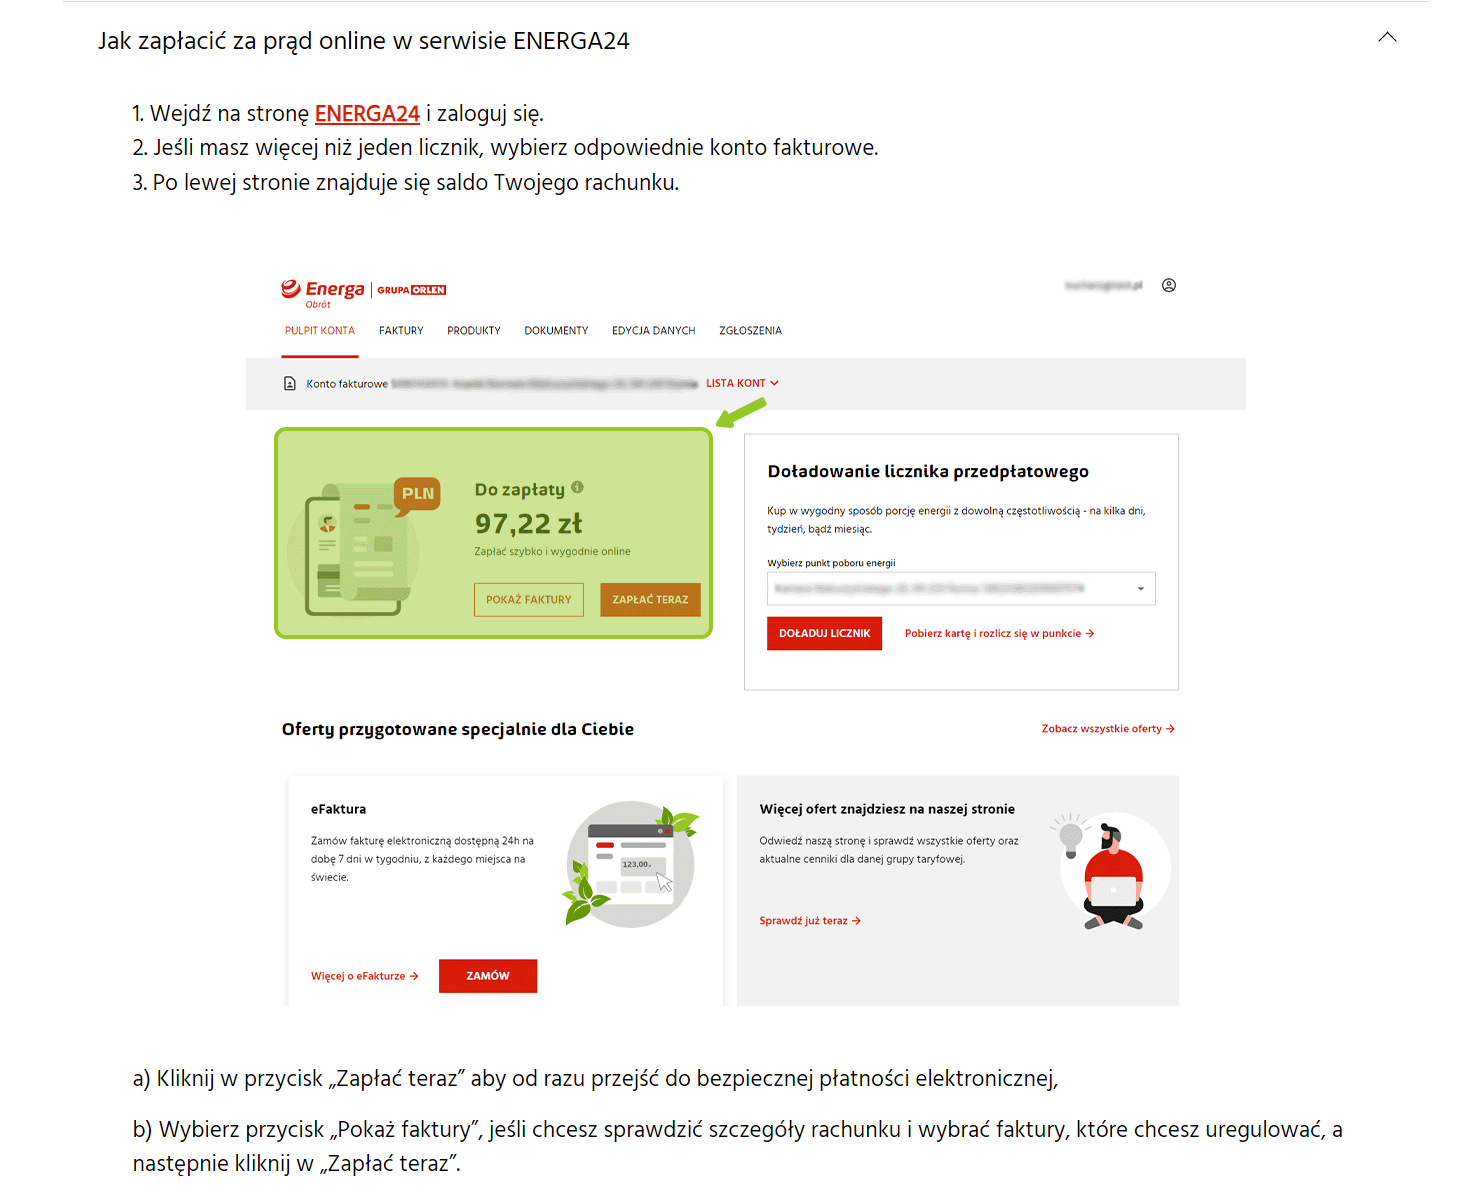
\includegraphics[width=0.85\linewidth]{rys01/energa_manual_1.png} \\[-1ex]
		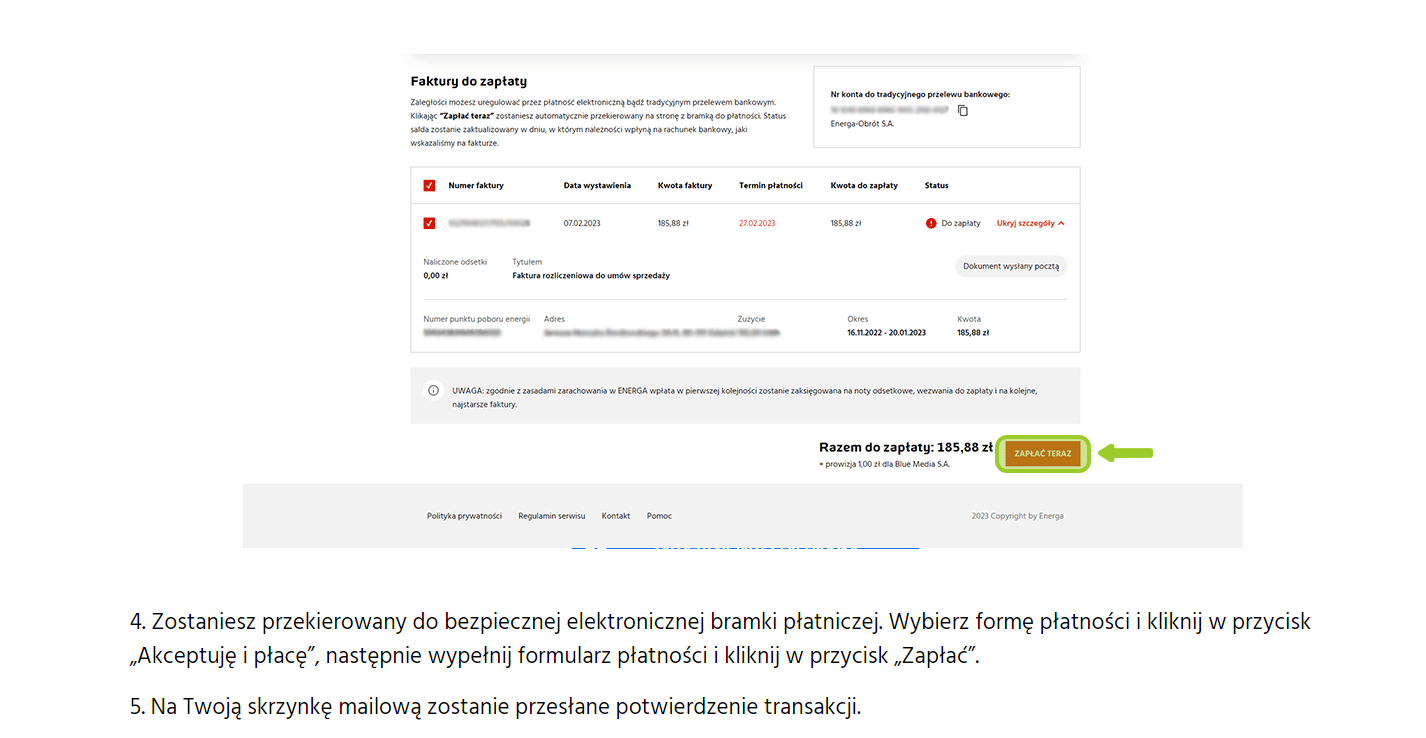
\includegraphics[width=0.85\linewidth]{rys01/energa_manual_2.png} \\[-1ex]
		\caption{Opis scenariusza dokonania płatności za energię elektryczną w serwisie ,,Energa24''~\cite{energa}}
	\label{fig:energa_manual}
\end{figure}

Innym przykładem systemu eBOK jest rozwiązanie dostarczane przez operatora telekomunikacji Play, który umożliwia użytkownikom zarządzanie usługami telekomunikacyjnymi oraz multimediami. System ,,Play24'' oferuje szeroki zakres funkcji, takich jak monitorowanie zużycia internetu, minut rozmów czy SMS-ów, co pozwala użytkownikom na bieżąco śledzić stan swoich pakietów i w razie potrzeby dokupować dodatkowe usługi. Użytkownicy mogą również sprawdzać historię swoich aktywności, w tym szczegółowe informacje na temat wysyłanych wiadomości, połączeń czy zakupionych pakietów ~\cite{Play24}.

System ,,Play24'' pozwala także na łatwe i szybkie regulowanie płatności za usługi telekomunikacyjne, oferując różnorodne metody płatności, w tym Google Pay, Apple Pay oraz BLIK. Użytkownicy mogą skonfigurować automatyczne płatności, co znacząco upraszcza zarządzanie opłatami. Dodatkowo, aplikacja umożliwia dostęp do szczegółowych faktur oraz wyciągów z historii transakcji, co ułatwia kontrolowanie bieżących wydatków.

Co więcej, system ten umożliwia zarządzanie usługami światłowodowymi, w tym zdalne restartowanie routera czy zmianę hasła do Wi-Fi. W przypadku problemów technicznych, użytkownicy mogą zgłaszać usterki i diagnozować problemy bezpośrednio z poziomu aplikacji. Dzięki intuicyjnemu interfejsowi, użytkownicy mogą szybko przemieszczać się między funkcjami aplikacji, co znacząco usprawnia zarządzanie usługami telekomunikacyjnymi i technicznymi.

Rysunek \ref{fig:play24_manual} ilustruje te funkcje, jak użytkownicy mogą śledzić swoje zużycie internetu, zarządzać opłatami oraz kontrolować ustawienia sieci domowej, co zwiększa ich komfort użytkowania oraz zapewnia większą kontrolę nad korzystaniem z usług.

\begin{figure}[ht]
    \centering
    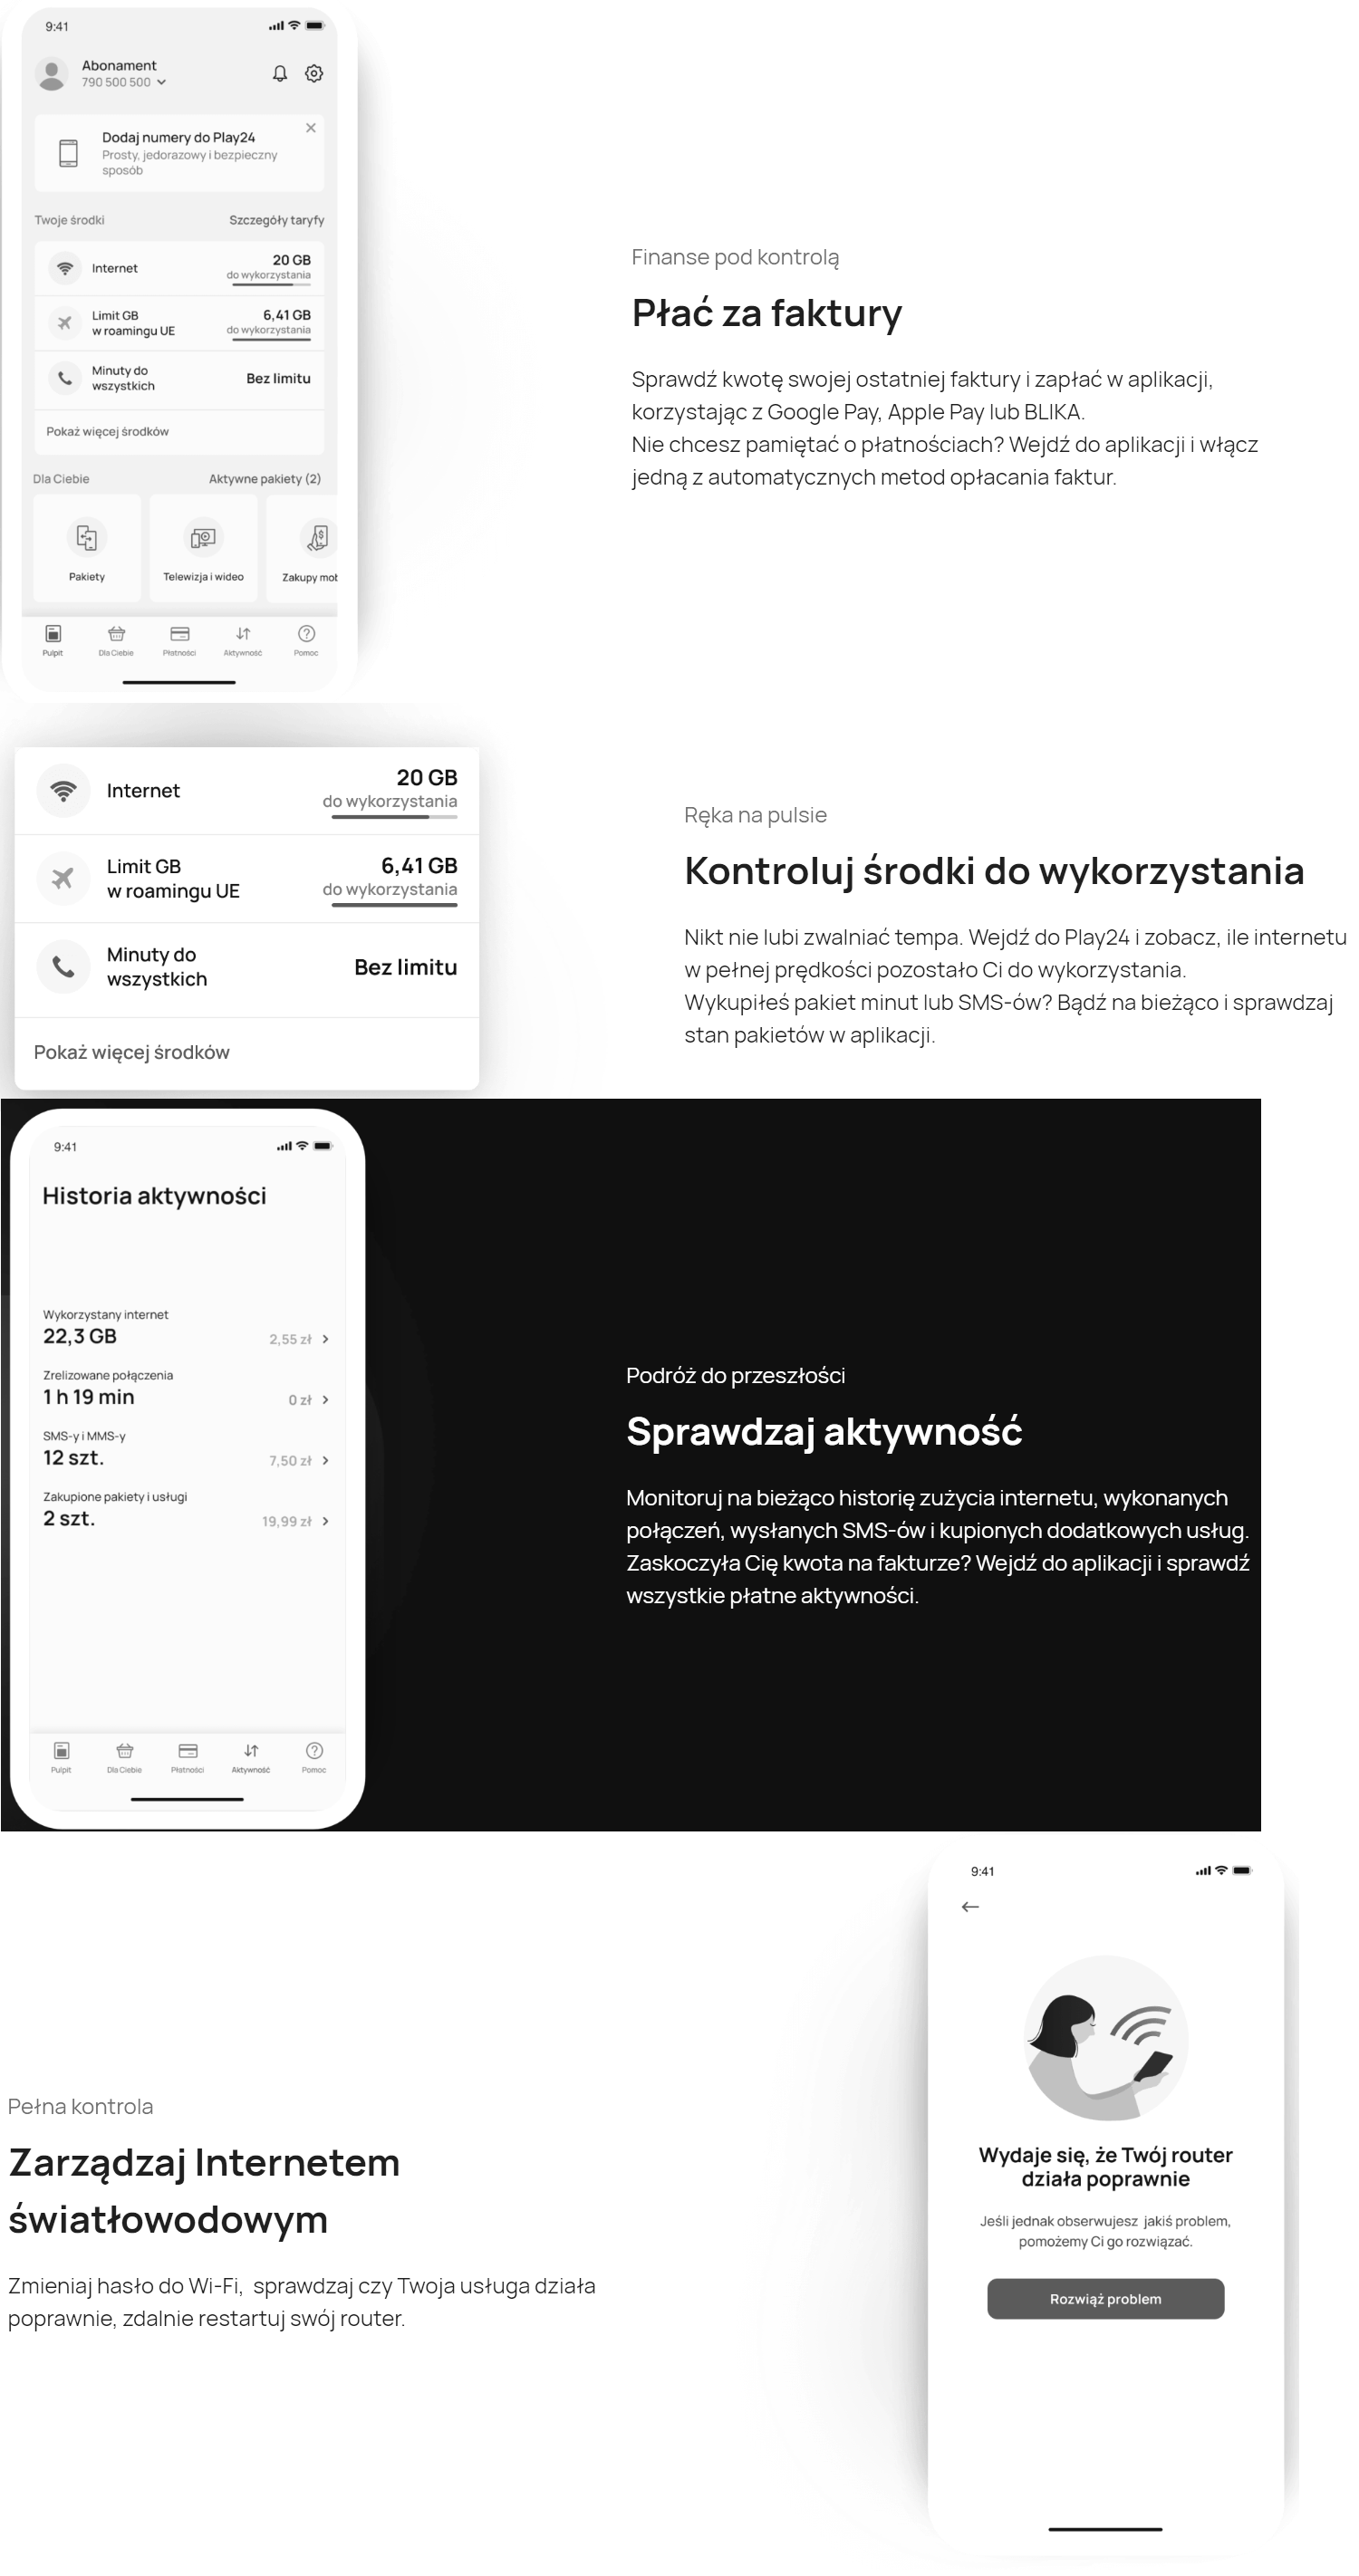
\includegraphics[width=0.6\linewidth]{rys01/play_manual}
    \caption{Opis głównych funkcji oferowanych w systemie ,,Play24''}
    \label{fig:play24_manual}
\end{figure}

Dostępne są również rozwiązania dostosowane specjalnie do potrzeb spółdzielni i wspólnot mieszkaniowych. Przykładem może być system ,,e-Kartoteka'', który umożliwia mieszkańcom zarządzanie zgłoszeniami usterek oraz podgląd postępu zgłoszenia, wgląd oraz regulację w płatności za nieruchomość, wgląd w dokumenty nieruchomości oraz wspólnoty, głosowanie nad uchwałami wspólnoty, a także komunikację z zarządem~\cite{e-kartoteka}. System ten oferuje również możliwość przeglądania rozliczeń mediów, takich jak woda, energia elektryczna czy ogrzewanie, co ułatwia mieszkańcom śledzenie swoich bieżących opłat i zużycia. Aplikacja ,,e-Kartoteka'' umożliwia również mieszkańcom szybki dostęp do wyciągów z rachunków i opłat miesięcznych, w tym szczegółowych rozliczeń za media (patrz rysunek~\ref{fig:kartoteka_manual}). Dzięki intuicyjnemu interfejsowi użytkownicy mogą sprawnie poruszać się między funkcjami, takimi jak tablica ogłoszeń, forum dyskusyjne dla mieszkańców czy dokumentacja nieruchomości, co znacząco poprawia komunikację i współpracę w obrębie wspólnoty. Ponadto mieszkańcy mają możliwość zgłaszania odczytów liczników, co automatycznie generuje informacje na temat aktualnego stanu rozliczeń oraz zaległych opłat, podobnie jak widoczne na przedstawionym obrazie funkcje raportowania stanu liczników i przeglądania historii faktur.
\begin{figure}[ht]
    \centering
    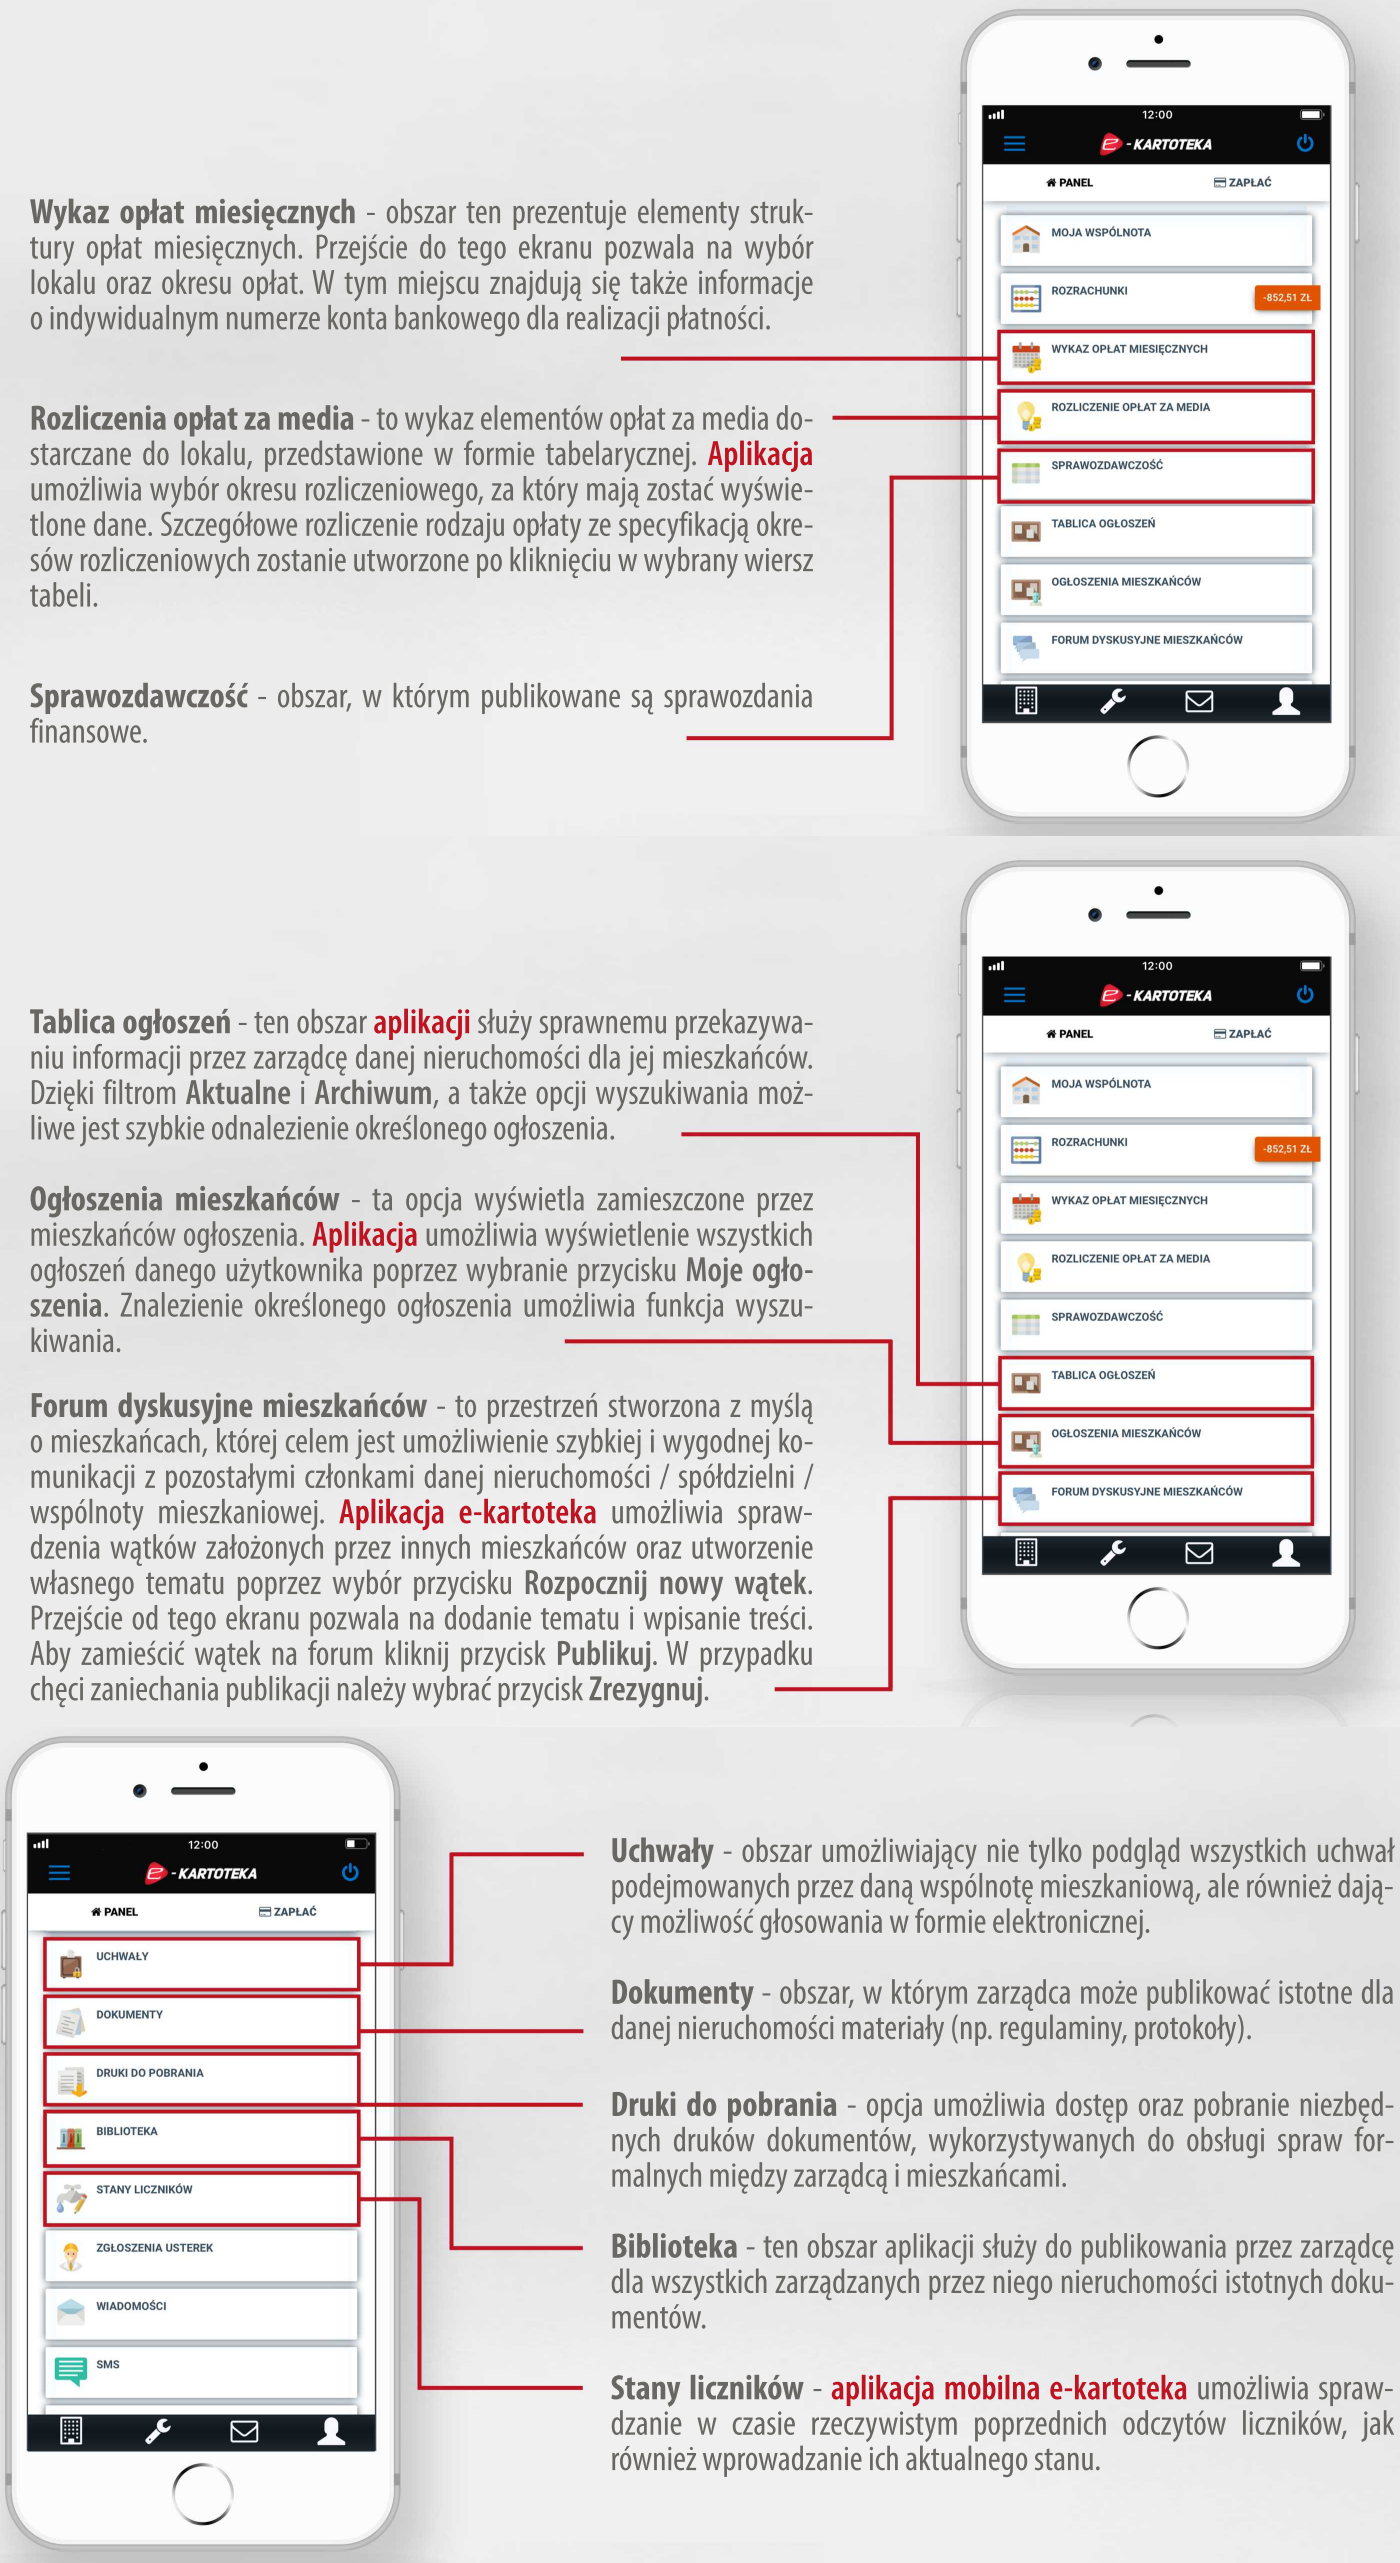
\includegraphics[width=0.6\linewidth]{rys01/kartoteka_manual}
    \caption{Opis głównych funkcji oferowanych w systemie ,,e-Kartoteka''~\cite{e-kartoteka_manual}}
    \label{fig:kartoteka_manual}
\end{figure}

Systemy eBOK różnią się pod względem funkcji, skalowalności oraz stopnia integracji z innymi rozwiązaniami, takimi jak narzędzia płatności online, systemy zarządzania nieruchomościami czy aplikacje mobilne. Wybór odpowiedniego systemu zależy od potrzeb operacyjnych organizacji, liczby użytkowników oraz poziomu automatyzacji procesów. Wdrożenie eBOK-ów wymaga przemyślanego doboru technologii i architektury, co wiąże się z licznymi wyzwaniami. Projektowanie tych systemów stanowi okazję do rozwijania umiejętności programistycznych, automatyzacji procesów i zarządzania projektami IT. Niniejsza praca koncentruje się na rozwiązaniu problemu automatyzacji obsługi wspólnot mieszkaniowych oraz usprawnieniu komunikacji między mieszkańcami a administracją.

Celem niniejszej pracy inżynierskiej jest zaprojektowanie i wdrożenie aplikacji eBOK dla wspólnoty mieszkaniowej. Wybór tego rozwiązania wynika z potrzeby automatyzacji procesów obsługi mieszkańców oraz poprawy komunikacji między mieszkańcami a administracją. Nowoczesne systemy eBOK eliminują konieczność bezpośredniego kontaktu, umożliwiając załatwienie większości spraw online, co zwiększa wygodę, oszczędność czasu oraz bezpieczeństwo transakcji i wymiany informacji.

Finalny produkt opracowywany w tej pracy nosi nazwę „Harmony Home Net”, odzwierciedlając kluczowe cele aplikacji: ułatwienie komunikacji i współpracy między mieszkańcami a administracją oraz zapewnienie płynnego i zintegrowanego zarządzania nieruchomościami.

\section{Cel i zakres pracy}

Celem niniejszej pracy jest zaprojektowanie i wdrożenie internetowej aplikacji elektronicznego biura obsługi klienta (eBOK) dla wspólnoty mieszkaniowej. Aplikacja ma na celu ułatwienie zarządzania procesami związanymi z komunikacją, płatnościami, zgłoszeniami technicznymi oraz dostępem do dokumentów. Dzięki temu zarówno mieszkańcy, jak i administratorzy będą mogli korzystać z kompleksowego narzędzia, które ma automatyzować wiele codziennych zadań i zwiększać efektywność zarządzania wspólnotą.

Zakres prac obejmuje pełny cykl rozwoju oprogramowania, od analizy potrzeb wspólnoty, poprzez projektowanie architektury systemu, aż po wdrożenie i przetestowanie gotowego rozwiązania. Analiza wymagań obejmie zarówno potrzeby funkcjonalne, jak i niefunkcjonalne, takie jak bezpieczeństwo, wydajność oraz integracja z zewnętrznymi systemami. Projektowanie uwzględnia iteracyjne testowanie oraz możliwość dalszego rozszerzania systemu o nowe moduły funkcjonalne.

Aplikacja będzie dostępna w przeglądarce internetowej i zoptymalizowana pod kątem dostępu z różnych urządzeń, w tym także w wersji desktopowej. Backend systemu zostanie stworzony w technologii Java i Spring Boot, co umożliwi budowę skalowalnych, bezpiecznych i łatwych w utrzymaniu aplikacji. Baza danych PostgreSQL będzie działać jako obraz Dockerowy, co zapewni izolację środowiska oraz ułatwi wdrażanie, zarządzanie i skalowanie aplikacji~\cite{EARTHLY}.

Frontend aplikacji zostanie zaprojektowany w języku TypeScript z wykorzystaniem frameworka Next.js, co pozwoli na stworzenie nowoczesnego, responsywnego interfejsu użytkownika, zapewniającego intuicyjną obsługę oraz szybkie działanie systemu.

\section{Układ pracy}
% tutaj opis zawartości kolejnych rozdziałów, można zredagować na końcu
\chapter{Analiza wymagań}

Analiza wymagań to kluczowy etap procesu tworzenia oprogramowania, który ma na celu zrozumienie potrzeb użytkowników oraz specyfikacji systemu. W przypadku projektowania aplikacji typu Elektroniczne Biuro Obsługi Klienta (eBOK) dla wspólnoty mieszkaniowej, istotne jest zidentyfikowanie wszystkich funkcji, 
% TO DO: proszę w miarę możliwości unikać wyrażenia "funkcjonalności", a używać raczej "funkcje".
które będą odpowiadały zarówno mieszkańcom, jak i administratorom. Poprawna analiza wymagań pozwala na stworzenie systemu, który nie tylko spełnia potrzeby użytkowników, ale także jest skalowalny, bezpieczny i łatwy w utrzymaniu.

W niniejszym rozdziale zostaną omówione zarówno funkcjonalne, jak i niefunkcjonalne wymagania systemu, uwzględniając różnorodne potrzeby użytkowników. Przeanalizowane zostaną także kluczowe aspekty, takie jak bezpieczeństwo, wydajność, intuicyjność interfejsu, a także integracja z innymi systemami. Wymagania te będą stanowiły podstawę do zaprojektowania architektury systemu oraz jego implementacji.

\section{Opis architektury systemu}
Opis architektury systemu jest kluczowym krokiem w projektowaniu oprogramowania, który pozwala na stworzenie efektywnego i funkcjonalnego rozwiązania. W przypadku aplikacji Elektronicznego Biura Obsługi Klienta (eBOK) dla wspólnoty mieszkaniowej, architektura musi uwzględniać zarówno potrzeby użytkowników, jak i wymagania techniczne. W tym rozdziale przedstawione zostaną główne komponenty systemu oraz ich wzajemne interakcje, na podstawie przedstawionego schematu.

\begin{figure}[ht]
    \centering
    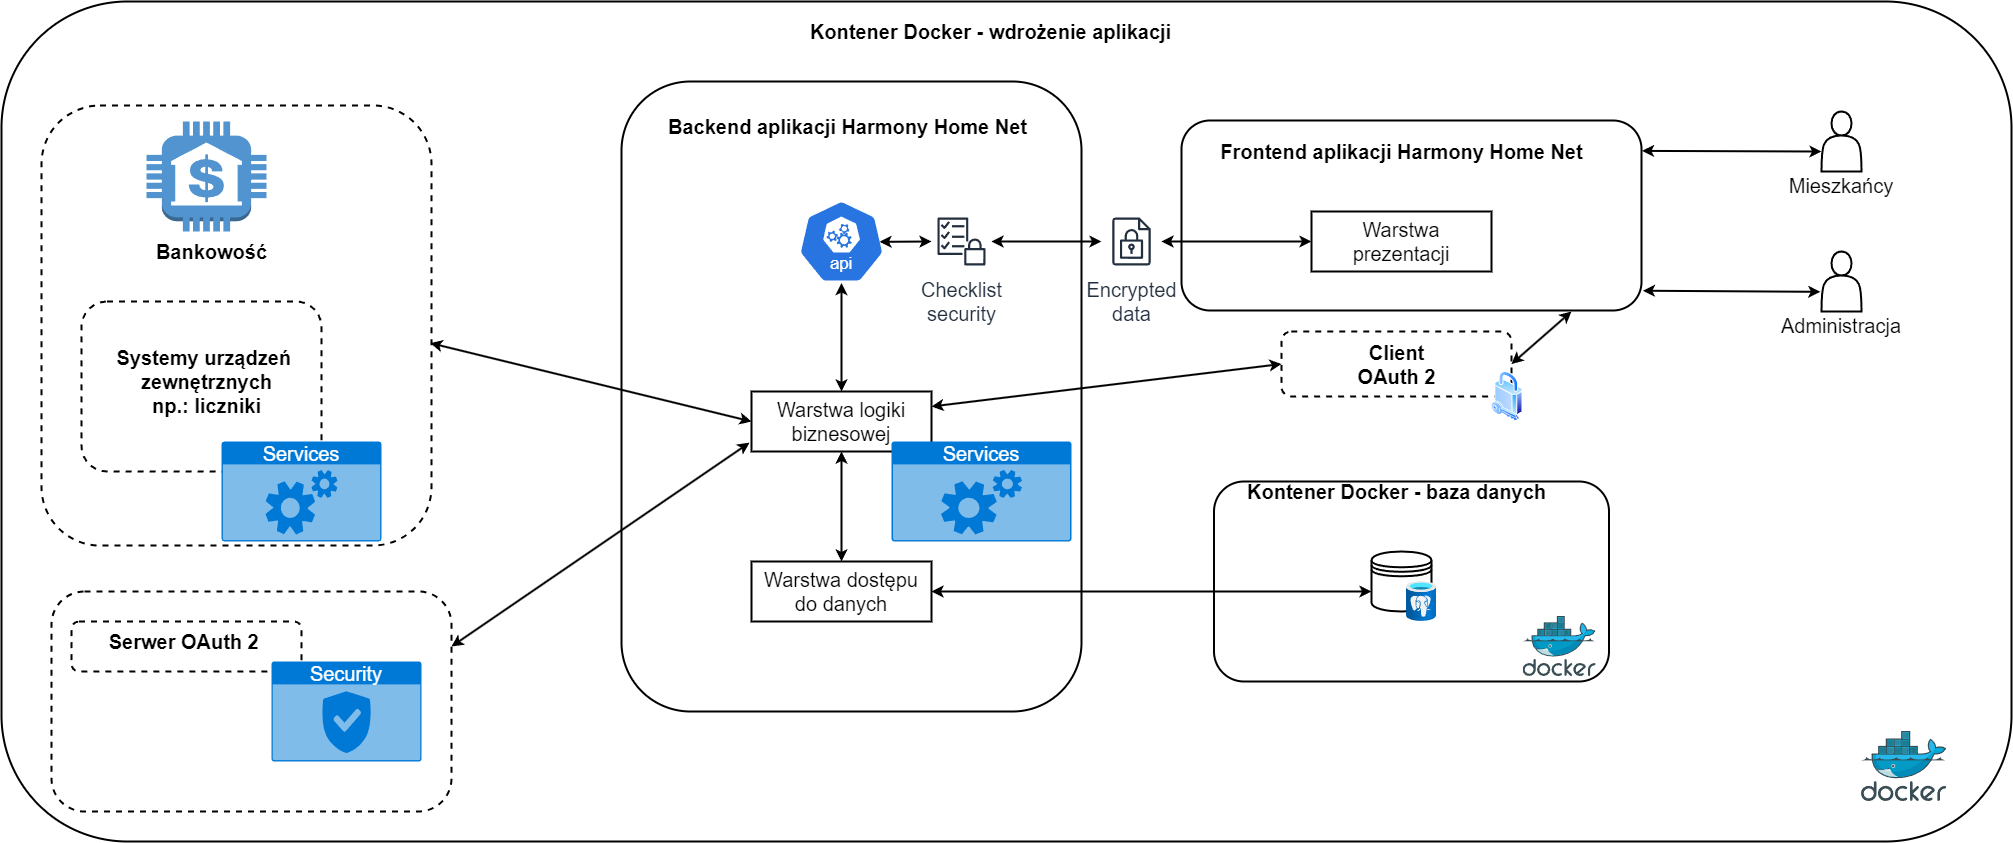
\includegraphics[width=1.11\linewidth]{Schematy/zarys_architektury.png}
    \caption{Diagram przedstawiający architekturę systemu „Harmony Home Net”}
    \label{fig:zarys_architektury}
\end{figure}


\subsection{Komponenty systemu}

Jak przedstawiono na rysunku \ref{fig:zarys_architektury}, system składa się z kilku kluczowych komponentów, które współpracują ze sobą, aby zapewnić pełną integralność aplikacji.

\begin{itemize} 

	\item \textbf{Frontend} - Interfejs użytkownika aplikacji, zrealizowany w frameworku Next.js, pisany w TypeScript. Frontend obsługuje interakcje użytkowników (mieszkańców oraz administratorów) oraz prezentuje dane w odpowiednim formacie. Komunikacja z backendem odbywa się za pośrednictwem bezpiecznego protokołu HTTPS, a dane są szyfrowane przy pomocy protokołu TLS. Frontend (pokazany po prawej stronie na rys. \ref{fig:zarys_architektury}) pełni kluczową rolę w interakcji z użytkownikami, umożliwiając im dostęp do danych w łatwy sposób.

	\item \textbf{Backend} - Serwer aplikacji, oparty na Spring Boot, działający w kontenerze Docker, odpowiedzialny za logikę biznesową oraz zarządzanie danymi. Backend znajduje się centralnie na diagramie (rys. \ref{fig:zarys_architektury}) i odpowiada za funkcje takie jak autoryzacja użytkowników (przez OAuth 2.0), obsługa zgłoszeń mieszkańców, zarządzanie płatnościami i komunikacja z zewnętrznymi systemami. Konteneryzacja za pomocą Dockera (również widoczna na diagramie) zapewnia elastyczność i łatwość w skalowaniu.

	\item \textbf{Warstwa logiki biznesowej} - Kluczowa część backendu odpowiedzialna za implementację reguł biznesowych, która obsługują funkcje aplikacji, takie jak przetwarzanie zgłoszeń czy zarządzanie danymi użytkowników. Logika biznesowa, choć nie jest wyodrębniona na diagramie, stanowi centralną część backendu, odpowiadając za koordynację przepływu danych między frontendem, bazą danych oraz systemami zewnętrznymi.

	\item \textbf{Warstwa dostępu do danych} - Odpowiada za komunikację z bazą danych PostgreSQL, przechowującą informacje dotyczące użytkowników, zgłoszeń, płatności i innych istotnych danych. Ta warstwa zapewnia trwałość i integralność danych w systemie. W diagramie (rys. \ref{fig:zarys_architektury}), baza danych PostgreSQL jest zlokalizowana po prawej stronie, gdzie przechowuje wszystkie kluczowe informacje aplikacji.

	\item \textbf{Baza danych} - System PostgreSQL, działający w kontenerze Docker, przechowuje wszystkie kluczowe dane aplikacji. Dzięki konteneryzacji możliwe jest łatwe skalowanie i zarządzanie bazą danych w środowisku produkcyjnym. Baza danych jest przedstawiona po prawej stronie diagramu, gdzie współpracuje z backendem przy operacjach odczytu i zapisu danych.

	\item \textbf{Serwer OAuth 2.0} - Serwer autoryzacji, który zapewnia bezpieczeństwo dostępu do zasobów systemu przez użytkowników. OAuth 2.0 umożliwia zarządzanie autoryzacją dostępu, co zwiększa bezpieczeństwo aplikacji. Na diagramie nie jest bezpośrednio zaznaczony, ale stanowi część systemu bezpieczeństwa aplikacji.

	\item \textbf{Systemy zewnętrzne} - Aplikacja integruje się z zewnętrznymi systemami, takimi jak bankowość (np. obsługa płatności online) oraz urządzenia zewnętrzne (np. liczniki zużycia mediów), co umożliwia kompleksową obsługę mieszkańców i automatyzację procesów. Zewnętrzne systemy znajdują się po lewej stronie diagramu, skąd integrują się z backendem w celu wymiany danych.


\end{itemize}

\subsection{Interakcje między komponentami}

Interakcje między komponentami są kluczowe dla sprawnego funkcjonowania systemu. W architekturze tej wykorzystano konteneryzację przy pomocy Dockera, co umożliwia izolowanie poszczególnych elementów systemu oraz ułatwia to skalowanie.

\begin{itemize} 
	\item \textbf{Frontend i Backend} - Frontend wysyła zapytania HTTPS do backendu (pokazanego pośrodku diagramu rys. \ref{fig:zarys_architektury}), poprzez zabezpieczenie protokołem TLS, w celu pobrania lub wysłania w sposób bezpieczny danych. Backend przetwarza te zapytania, wykonuje odpowiednie operacje na bazie danych i zwraca odpowiedzi do frontendu. Dane są wysyłane i odbierane w formacie JSON. Te interakcje są widoczne na schemacie jako przepływ między frontem po prawej a backendem w centrum.
	
	\item \textbf{Backend i Baza danych} - Backend łączy się z bazą danych PostgreSQL w celu odczytu i zapisu danych. Wszystkie operacje na danych, takie jak dodawanie nowych zgłoszeń czy aktualizacja informacji o płatnościach, są realizowane przez backend.

	\item \textbf{Backend i System płatności} - Backend integruje się z systemami płatności, aby obsługiwać transakcje finansowe. Po dokonaniu płatności, system płatności przekazuje informacje zwrotne do backendu, który aktualizuje status płatności w bazie danych.

	\item \textbf{Backend i System powiadomień} - Backend wysyła powiadomienia do systemu powiadomień w celu informowania użytkowników o ważnych zdarzeniach. System powiadomień następnie dostarcza te informacje do użytkowników za pomocą e-maili lub SMS-ów.

\end{itemize}


\section{Wymagania aplikacji}

Aplikacja eBOK (Elektroniczne Biuro Obsługi Klienta) jest narzędziem wspierającym zarządzanie wspólnotami mieszkaniowymi, które ma na celu poprawę komunikacji pomiędzy mieszkańcami a administracją oraz automatyzację procesów związanych z obsługą nieruchomości. Jednym z kluczowych aspektów aplikacji jest zarządzanie lokalami, które w systemie pełnią centralną rolę, gdyż każda funkcja aplikacji – od zgłaszania usterek, przez płatności, po głosowania – jest związana z konkretnym lokalem.

Lokale, czyli nieruchomości (mieszkania, apartamenty, biura itp.), są podstawowym zasobem, który wymaga skutecznego zarządzania zarówno z perspektywy mieszkańca, jak i administratora. Dla mieszkańca lokal jest miejscem, do którego przypisane są należności finansowe, zgłoszenia techniczne czy dokumenty. Z perspektywy administratora, każdy lokal stanowi jednostkę, którą należy nadzorować pod kątem bieżących płatności, obsługi technicznej, jak również interakcji z właścicielami i najemcami. Dlatego zarządzanie lokalami/nieruchomościami w aplikacji eBOK jest jedną z kluczowych funkcji, zapewniającą przejrzystość oraz efektywność administracji.

\subsection{Przykłady użycia aplikacji}

Aplikacja eBOK oferuje różnorodne przypadki użycia, które ilustrują funkcje dostępne dla różnych grup użytkowników. Głównym obszarem jej zastosowania jest zarządzanie relacją pomiędzy mieszkańcem a administratorem nieruchomości, w kontekście takich działań jak płatności, zgłoszenia usterek, dostęp do dokumentów czy udział w głosowaniach. W aplikacji będzie można wyodrębnić 2 główne grupy użytkowników:

\begin{itemize} 

	\item \textbf{Mieszkańcy (właściciele i najemcy):} logując się do systemu, mają możliwość sprawdzenia należności za lokal, uregulowania opłat online oraz przeglądania historii rachunków. Mogą również zgłaszać usterki dotyczące lokalu (np. przeciek, awaria ogrzewania) i śledzić status zgłoszenia. Dodatkowo, mieszkaniecy ma dostęp do dokumentów związanych z jego lokalem, takich jak umowy, regulaminy czy faktury.
	
	\item \textbf{Administratorzy:} za pomocą panelu administracyjnego zarządzają zgłoszeniami technicznymi, przypisując je do wykonawców. Odpowiadają również za monitorowanie płatności związanych z każdym lokalem, a także za prowadzenie rejestru dokumentów i interakcje z mieszkańcami.
	
\end{itemize}

Każda z tych grup użytkowników ma dostęp do odpowiednich funkcji aplikacji, które spełniają jej potrzeby.

\subsection{Wymagania funkcjonalne}

Wymagania funkcjonalne aplikacji eBOK skupiają się na kluczowych obszarach działalności, które odpowiadają za sprawne funkcjonowanie wspólnoty mieszkaniowej.

\begin{enumerate}[label=\arabic*.]

	\item \textbf{Zarządzanie kontem użytkownika i lokalami:} Użytkownicy muszą mieć możliwość tworzenia kont, zarządzania swoimi danymi osobowymi oraz przypisywania lokali do konta. Mieszkańcy mogą być przypisani do wielu lokali, w zależności od tego, czy są właścicielami, czy najemcami. Funkcje dostępne dla mieszkańca są zależne od jego roli w danym lokalu (właściciel będzie miał znacząco większą ilość dostępnych funkcji w porównaniu do najemcy).

	\item \textbf{Przegląd i płatność należności:} Mieszkańcy mogą przeglądać szczegółowe informacje na temat należności przypisanych do konkretnego lokalu, którym zarządzają. Właściciele mają dostęp do pełnej historii opłat oraz możliwość ich realizacji online. Najemcy mogą jedynie przeglądać należności powiązane z ich umową najmu. System umożliwia szybki dostęp do historii opłat oraz realizację płatności online. Powiadomienia o zaległościach związanych z danym lokalem przypominają o konieczności uregulowania zobowiązań.

	\item \textbf{Zarządzanie zgłoszeniami technicznymi dla lokali:} Mieszkańcy (zarówno właściciele, jak i najemcy) mogą zgłaszać problemy techniczne dotyczące lokali, z którymi są powiązani. Właściciele mogą mieć dodatkowe uprawnienia do nadzorowania zgłoszeń związanych z większą liczbą lokali.

	\item \textbf{Zarządzanie dokumentami:} Lokale są również powiązane z dokumentami, takimi jak umowy najmu, protokoły przekazania, regulaminy czy faktury. Właściciele mają pełen dostęp do dokumentów powiązanych z ich lokalami, a najemcy mogą przeglądać dokumenty dotyczące tylko ich umowy najmu. Administratorzy zarządzają tymi dokumentami, przypisując je odpowiednim użytkownikom.

	\item \textbf{Głosowania mieszkańców:} W przypadku istotnych decyzji dotyczących zarządzania wspólnotą, administrator może organizować głosowania. Prawo głosu przysługuje mieszkańcom przypisanym do danego lokalu na podstawie ich roli (właściciel). Dzięki aplikacji proces głosowania jest zautomatyzowany, a wyniki są dostępne w czasie rzeczywistym.

	\item \textbf{Powiadomienia i komunikacja:} System powiadomień informuje użytkowników o ważnych wydarzeniach związanych z ich lokalem, takich jak zaległe płatności, zgłoszenia serwisowe czy nadchodzące głosowania. Rola użytkownika (właściciel lub najemca) determinuje, jakie powiadomienia są wysyłane oraz do których funkcji ma dostęp.

	\item \textbf{Panel administracyjny:} Administratorzy korzystają z zaawansowanego panelu, który pozwala im zarządzać wszystkimi lokalami, przypisywać mieszkańców do lokali, weryfikować uprawnienia użytkowników oraz monitorować zgłoszenia techniczne. Na podstawie umów lub dokumentów, administrator przypisuje lokale do nowych i istniejących kont mieszkańców.

	\item \textbf{Integracja z zewnętrznymi systemami:} Aplikacja eBOK musi umożliwiać integrację z systemami takimi jak systemy pomiarowe liczników mediów (np. wodomierze, liczniki energii) oraz systemy płatności. Taka integracja usprawnia zarządzanie lokalami, umożliwiając automatyczne generowanie rachunków oraz synchronizację danych dotyczących zużycia mediów.

	\item \textbf{Stany liczników:} System powinien umożliwiać użytkownikom wprowadzanie oraz przeglądanie stanów liczników powiązanych z danym lokalem, takich jak odczyty wodomierzy czy liczników energii. Aplikacja powinna automatycznie generować rozliczenia na podstawie wprowadzonych odczytów, co pozwala na dokładniejsze monitorowanie zużycia mediów oraz zarządzanie opłatami. Właściciele lokali mogą także mieć możliwość przeglądania historii odczytów i analizowania tendencji zużycia w czasie, co pomoże im lepiej planować wydatki i kontrolować koszty związane z mediami.
	
	\item \textbf{Forum mieszkańców:} System umożliwia utworzenie forum dyskusyjnego dla mieszkańców. Każdy mieszkaniec przypisany do lokalu, niezależnie od roli (właściciel, najemca), ma możliwość wzięcia udziału w dyskusjach, dodawania nowych tematów, odpowiadania na pytania innych mieszkańców oraz dzielenia się opiniami na temat zarządzania nieruchomościami, zgłoszeń technicznych czy innych spraw związanych ze wspólnotą. Administratorzy mogą moderować forum, usuwając nieodpowiednie treści oraz przypinając istotne informacje.


\end{enumerate}


\subsection{Wymagania niefunkcjonalne}

\begin{enumerate}[label=\arabic*.] 

	\item \textbf{Skalowalność:} System musi być na tyle elastyczny, aby mógł obsługiwać zarówno małe wspólnoty mieszkaniowe, jak i większe spółdzielnie, z możliwością zarządzania setkami lub tysiącami lokali aby obsłużyć rosnącą liczbę użytkowników oraz lokali bez znaczących spadków wydajności. Zastosowanie technologii Docker do konteneryzacji backendu i bazy danych PostgreSQL umożliwia łatwe skalowanie poziome (dodawanie kolejnych instancji), co pozwala na rozdzielenie obciążenia na większą liczbę serwerów.

	\item \textbf{Bezpieczeństwo:} Wszystkie dane użytkowników muszą być przechowywane i przesyłane w sposób bezpieczny. Wymagane jest szyfrowanie komunikacji między frontendem a backendem (TLS), a także autoryzacja użytkowników za pomocą OAuth 2.0. Ponadto system musi chronić dane przed nieautoryzowanym dostępem, co obejmuje zabezpieczenia na poziomie aplikacji, takie jak ograniczenie dostępu do funkcji na podstawie roli użytkownika (np. właściciel, najemca, administrator).

	\item \textbf{Wydajność:} System powinien być responsywny, zapewniając jak najszybszy możliwy czas odpowiedzi na zapytanie. Backend oparty na Spring Boot oraz baza danych PostgreSQL muszą być odpowiednio zoptymalizowane pod kątem operacji zapisu i odczytu, aby sprostać wymaganiom w czasie rzeczywistym, szczególnie podczas obciążeń związanych z masowym przetwarzaniem danych (np. zgłoszenia techniczne, płatności).

	\item \textbf{Dostępność:} Aplikacja powinna być dostępna przez 99,9\% czasu, z minimalnymi przerwami na konserwację. Wdrożenie technologii kontenerowej (Docker) oraz monitorowanie serwerów w czasie rzeczywistym pozwala na szybkie identyfikowanie problemów i automatyczne odzyskiwanie usług w przypadku awarii.

	\item \textbf{Intuicyjność interfejsu:} Aplikacja musi być łatwa w obsłudze zarówno dla mieszkańców, jak i administratorów. Intuicyjny interfejs, oparty na komponentach Shadcn UI i zgodny z wytycznymi WCAG 2.0, zapewnia łatwy dostęp do funkcji. Ocenę intuicyjności można przeprowadzić na podstawie testów akceptacyjnych, w których użytkownicy będą oceniali łatwość korzystania z systemu w skali.
	
	\item \textbf{Zgodność z przepisami RODO:} System musi spełniać wymagania dotyczące ochrony danych osobowych, wynikające z RODO. Oznacza to, że wszystkie dane osobowe przechowywane w systemie muszą być chronione, użytkownicy muszą mieć możliwość wglądu w swoje dane, ich modyfikacji, a także żądania ich usunięcia. Przetwarzanie danych osobowych musi być odpowiednio udokumentowane, a dostęp do tych danych powinien być ograniczony.

	\item \textbf{Niezawodność:} System musi zapewniać ciągłość działania oraz zachowywać dane użytkowników nawet w przypadku awarii serwera. Konieczne jest wdrożenie mechanizmów regularnych kopii zapasowych bazy danych oraz planu odzyskiwania po awarii, który umożliwia szybkie przywrócenie systemu do pełnej funkcjonalności w krótkim czasie.

	\item \textbf{Testowalność:} Każda z funkcji aplikacji powinna być możliwa do przetestowania w sposób automatyczny, co umożliwi szybkie wykrywanie błędów w kodzie. Testy automatyczne powinny obejmować testy jednostkowe, integracyjne oraz systemowe, sprawdzając poprawność działania każdej funkcji zarówno z poziomu frontendu, jak i backendu. Testy akceptacyjne powinny obejmować scenariusze użytkownika, weryfikując, czy system spełnia wymagania stawiane przez administratorów i mieszkańców.

	\item \textbf{Elastyczność:} System powinien umożliwiać łatwe wprowadzanie nowych funkcji lub modyfikację istniejących bez konieczności przeprowadzania szerokich zmian w kodzie. Architektura warstwowa (N-tier), z wyraźnym rozdzieleniem logiki biznesowej, danych oraz interfejsu użytkownika, zapewnia elastyczność oraz ułatwia przyszły rozwój aplikacji.
	
\end{enumerate}

\section{Podsumowanie}

Analiza wymagań dla systemu „Harmony Home Net” jest kluczowym krokiem w kierunku zaprojektowania i implementacji aplikacji, która sprosta potrzebom zarówno mieszkańców, jak i administratorów wspólnot mieszkaniowych. Wymagania funkcjonalne i niefunkcjonalne omówione w tym rozdziale stanowią podstawę do dalszego projektowania systemu oraz planowania jego architektury. Umożliwiają one stworzenie aplikacji, która będzie nie tylko spełniać oczekiwania użytkowników, ale także zapewniać wysoki poziom bezpieczeństwa, wydajności i skalowalności, niezbędnych do efektywnego zarządzania nieruchomościami.

\chapter{Implementacja}
% TO DO: dodać jakieś zagajenie

\chapter{Podsumowanie pracy}

Niniejsza praca dyplomowa przedstawia proces projektowania i implementacji systemu „Harmony Home Net” – aplikacji typu eBOK dedykowanej wspólnotom mieszkaniowym. Głównym celem projektu było stworzenie rozwiązania wspierającego zarządzanie wspólnotami, komunikację pomiędzy mieszkańcami a administracją oraz automatyzację kluczowych procesów związanych z obsługą nieruchomości. Poniżej podsumowano kluczowe aspekty realizacji tego przedsięwzięcia.

\section{Zakres i wynik projektu}
W pracy przedstawiono pełny cykl życia oprogramowania, począwszy od analizy wymagań funkcjonalnych i niefunkcjonalnych, poprzez projektowanie architektury, aż po implementację i testy prototypu. System został zaprojektowany w oparciu o nowoczesne technologie, takie jak:
\begin{itemize}
    \item \textbf{Backend:} Spring Boot -- zapewniający elastyczność, bezpieczeństwo i wydajność aplikacji,
    \item \textbf{Frontend:} Next.js -- umożliwiający responsywność interfejsu i optymalizację SEO,
    \item \textbf{Baza danych:} PostgreSQL -- gwarantująca integralność i spójność danych,
    \item \textbf{Konteneryzacja:} Docker -- wspierający skalowalność i łatwość wdrażania systemu.
\end{itemize}

Stworzony system oferuje szereg funkcji dostosowanych do potrzeb mieszkańców, administracji i administratorów:
\begin{itemize}
    \item \textbf{Zarządzanie użytkownikami} -- Kompleksowy system ról i poziomów dostępu,
    \item \textbf{Obsługa płatności} -- Możliwość przeglądania należności, realizacji płatności online oraz harmonogramowania przypomnień,
    \item \textbf{Zgłoszenia techniczne} -- Funkcja zgłaszania i monitorowania usterek,
    \item \textbf{Zarządzanie dokumentami} -- Dostęp do umów, regulaminów i faktur,
    \item \textbf{Głosowania} -- Mechanizmy organizacji głosowań i walidacji wyników,
    \item \textbf{Forum mieszkańców} -- Uproszczona platforma komunikacji wspólnoty.
\end{itemize}

\section{Wnioski}
System „Harmony Home Net” stanowi solidną bazę do rozwoju nowoczesnych aplikacji wspierających obsługę wspólnot mieszkaniowych. Realizacja tego projektu umożliwiła zdobycie praktycznych umiejętności w zakresie projektowania systemów informatycznych, integracji zewnętrznych usług oraz testowania oprogramowania. Ponadto, prototyp spełnia swoje założenia projektowe i jest gotowy do dalszego rozwijania w kierunku pełnoprawnej aplikacji produkcyjnej, która może znacząco poprawić efektywność zarządzania wspólnotami mieszkaniowymi. Rozwój ten może nastąpić w kilku kluczowych obszarach:
\begin{itemize}
    \item pełna integracja z zewnętrznymi systemami, np. bankowości czy urządzeń pomiarowych,
    \item rozbudowa funkcji analitycznych, takich jak generowanie zaawansowanych raportów,
    \item wdrożenie bardziej zaawansowanego interfejsu użytkownika dla mieszkańców,
    \item zwiększenie automatyzacji procesów poprzez implementację zaawansowanych mechanizmów opartych na diagramach BPMN.
\end{itemize}



\appendix
\chapter{Instrukcja wdrożeniowa}

W celu uruchomienia prototypu systemu „Harmony Home Net” przygotowano środowisko bazujące na technologii Docker, które umożliwia szybkie uruchomienie wszystkich niezbędnych komponentów, takich jak backend, frontend oraz baza danych. Poniżej przedstawiono szczegółowe wymagania i kroki związane z wdrożeniem.

\section{Wymagania wstępne}
Na maszynie wdrożeniowej powinny być zainstalowane:
\begin{itemize}
    \item Docker (wersja 20.10 lub nowsza),
    \item Docker Compose (wersja 1.29 lub nowsza),
    \item Konto Gmail skonfigurowane do wysyłania powiadomień (wymagane w prototypie).
\end{itemize}

\section{Konfiguracja środowiska}
Konfigurację kontenerów systemu zamieszczono w pliku \texttt{docker-compose.yml}. Kluczowe ustawienia obejmują:
\begin{itemize}
    \item konfigurację bazy danych PostgreSQL,
    \item uruchomienie backendu z podanymi zmiennymi środowiskowymi,
    \item uruchomienie frontendu w trybie deweloperskim,
    \item konfigurację narzędzia do zarządzania bazą danych (pgAdmin).
\end{itemize}

\begin{lstlisting}[language=yaml, caption=Fragment pliku \texttt{docker-compose.yml}]
version: '3.8'

services:
  backend_app:
    build:
      context: ./backend
    ports:
      - "8444:8443"
    depends_on:
      - db
    environment:
      # Database
      SPRING_DATASOURCE_URL: jdbc:postgresql://db:5432/HarmonyHomeNet_DB
      SPRING_DATASOURCE_USERNAME: user
      SPRING_DATASOURCE_PASSWORD: admin

      # Mail
      SPRING_MAIL_HOST: smtp.gmail.com
      SPRING_MAIL_PORT: 587
      SPRING_MAIL_USERNAME: your_email@example.com
      SPRING_MAIL_PASSWORD: yout_password

      # Super admin user details
      SUPER_ADMIN_FIRST_NAME: Daniel
      SUPER_ADMIN_LAST_NAME: Ryszkowski
      SUPER_ADMIN_EMAIL: daniel.hhn.SA@gmail.com
      SUPER_ADMIN_PASSWORD: superadmin_password123
      SUPER_ADMIN_PHONE: 111111111

  db:
    image: postgres:alpine
    ports:
      - "5433:5432"
    environment:
      POSTGRES_USER: user
      POSTGRES_PASSWORD: admin
      POSTGRES_DB: HarmonyHomeNet_DB
\end{lstlisting}

\subsection{Backend}

Dockerfile backendu został zaprojektowany zgodnie z dobrymi praktykami, co pozwala na tworzenie wieloetapowych obrazów. Pierwszy etap buduje aplikację, a drugi uruchamia ją w zoptymalizowanym środowisku.

\begin{lstlisting}[language=docker, caption=Dockerfile backendu]
FROM maven:3.8.5-openjdk-17 AS build
WORKDIR /backend_app
COPY pom.xml .
RUN mvn dependency:go-offline
COPY src ./src
RUN mvn package -DskipTests

FROM openjdk:17-jdk-alpine
WORKDIR /app
COPY --from=build /backend_app/target/*.jar app.jar
EXPOSE 8443
ENTRYPOINT ["java", "-jar", "app.jar", "--server.port=8443"]
\end{lstlisting}

\subsection{Frontend}

Dockerfile frontendu działa w trybie deweloperskim, co oznacza, że środowisko jest zoptymalizowane pod kątem prac rozwojowych. Mimo że takie podejście działa w prototypie, w przyszłości należy przygotować zoptymalizowaną wersję produkcyjną.

\begin{lstlisting}[language=docker, caption=Dockerfile frontendu]
FROM node:20-alpine
WORKDIR /app
COPY package*.json ./
RUN npm install
COPY . .
EXPOSE 3000
CMD npm run dev
\end{lstlisting}


\section{Przed pierwszym uruchomieniem}
\subsection{Zmienne środowiskowe}
Przed pierwszym uruchomieniem systemu należy skonfigurować zmienne środowiskowe, które definiują dane dostępowe do serwera pocztowego oraz informacje o koncie superadministratora. Są one zdefiniowane w sekcji \texttt{environment} pliku \texttt{docker-compose.yml}. Poniżej przedstawiono ich szczegóły:

\begin{lstlisting}[language=yaml, caption=Konfiguracja zmiennych środowiskowych]
# Mail
SPRING_MAIL_HOST: smtp.gmail.com
SPRING_MAIL_PORT: 587
SPRING_MAIL_USERNAME: your_email@example.com
SPRING_MAIL_PASSWORD: your_password

# Super admin user details
SUPER_ADMIN_FIRST_NAME: Daniel
SUPER_ADMIN_LAST_NAME: Ryszkowski
SUPER_ADMIN_EMAIL: daniel.hhn.SA@gmail.com
SUPER_ADMIN_PASSWORD: superadmin_password123
SUPER_ADMIN_PHONE: 111111111
\end{lstlisting}

\textbf{Opis pól do konfiguracji:}
\begin{itemize}
    \item \texttt{SPRING\_MAIL\_HOST}, \texttt{SPRING\_MAIL\_PORT} -- domyślne wartości dla serwera SMTP usługi Gmail.
    \item \texttt{SPRING\_MAIL\_USERNAME}, \texttt{SPRING\_MAIL\_PASSWORD} -- dane logowania do konta Gmail, które będzie wykorzystywane do wysyłania wiadomości e-mail. Wartości te należy uzupełnić własnym adresem e-mail i hasłem (lub hasłem aplikacji).
    \item \texttt{SUPER\_ADMIN\_FIRST\_NAME}, \texttt{SUPER\_ADMIN\_LAST\_NAME}, \texttt{SUPER\_ADMIN\_EMAIL}, \texttt{SUPER\_ADMIN\_PASSWORD}, \texttt{SUPER\_ADMIN\_PHONE} -- dane pierwszego użytkownika z rolą superadministratora. Wartości te można dostosować według potrzeb organizacji.
\end{itemize}

\subsection{Konfiguracja konta Gmail do wysyłania e-maili}
Aby system mógł korzystać z serwera Gmail do wysyłania wiadomości e-mail, należy skonfigurować konto Gmail zgodnie z poniższymi krokami:

\begin{enumerate}
    \item Zaloguj się na swoje konto Gmail.
    \item Przejdź do ustawień konta, a następnie wybierz sekcję \texttt{Bezpieczeństwo}.
    \item Włącz opcję \texttt{Dostęp mniej bezpiecznych aplikacji} (jeśli jest dostępna).
    \item Alternatywnie, jeżeli dostęp mniej bezpiecznych aplikacji nie jest dostępny, wygeneruj hasło aplikacji:
    \begin{itemize}
        \item Przejdź do sekcji \texttt{Hasła aplikacji}, przez wyszukiwarkę w panelu konta.
        \item Wybierz aplikację \texttt{Poczta} i urządzenie \texttt{Komputer}.
        \item Kliknij \texttt{Generuj} i skopiuj wygenerowane hasło.
        \item Wprowadź to hasło w polu \texttt{SPRING\_MAIL\_PASSWORD} w pliku \texttt{docker-compose.yml}.
    \end{itemize}
    \item \textbf{Upewnij się, że konto Gmail ma włączone uwierzytelnianie dwuskładnikowe, jeśli wymaga tego konfiguracja hasła aplikacji}.
\end{enumerate}

\section{Pierwsze uruchomienie systemu}
Po skonfigurowaniu zmiennych środowiskowych i konta Gmail, system można uruchomić za pomocą następującego polecenia:
\begin{verbatim}
docker-compose up --build
\end{verbatim}

W trakcie pierwszego uruchomienia backend automatycznie utworzy konto superadministratora z wykorzystaniem danych wprowadzonych w sekcji \texttt{SUPER\_ADMIN\_*} pliku \texttt{docker-compose.yml}. Konto to umożliwia dostęp do panelu administracyjnego aplikacji i zarządzanie systemem. Kod odpowiedzialny za inicjalizację prezentuje się następująco:
\begin{lstlisting}[language=Java, style=JavaStyle, caption=Kod inicjalizacji superadministratora]
@PostConstruct
public void init() {
    User superAdmin = createUserIfNotExists(
        superAdminFirstName,
        superAdminLastName,
        superAdminEmail,
        bCryptPasswordEncoder.encode(superAdminPassword),
        superAdminPhone,
        Role.ROLE_SUPER_ADMIN
    );
}
\end{lstlisting}

Po uruchomieniu:
\begin{itemize}
    \item Backend dostępny jest pod adresem \texttt{https://localhost:8444}.
    \item Frontend można otworzyć pod adresem \texttt{http://localhost:3000}.
    \item pgAdmin dostępny jest pod adresem \texttt{http://localhost:5050}.
\end{itemize}

\section{Uwagi i rozwój przyszłościowy}
Obecna implementacja frontendu w trybie deweloperskim działa poprawnie, ale wymaga optymalizacji przed wdrożeniem produkcyjnym. W przyszłości należy:
\begin{itemize}
    \item przygotować zoptymalizowaną wersję frontendu w trybie produkcyjnym,
    \item wdrożyć rzeczywistą integrację z zewnętrznymi systemami bankowymi i usługami SMS,
    \item rozszerzyć dokumentację wdrożeniową o instrukcje dotyczące monitorowania i skalowania aplikacji.
\end{itemize}

\chapter{Opis załączonej płyty CD/DVD}
\chapter{Krótki start}
Poniżej opisano prosty przypadek użycia aplikacji, w którym dodano nowego właściciela do systemu, następnie nowe mieszkanie, a na końcu przypisano właściciela do tego mieszkania.

\noindent \textbf{Logowanie i panel główny~~}
Aby skorzystać z systemu należy się do niego zalogować. Na rysunku~\ref{fig:logowanie} przedstawiono panel logowania do świeżo uruchomionego systemu w środowisku Docker. Dane do logowania, takie jak e-mail i hasło super administratora, są konfigurowane w pliku \texttt{docker-compose.yml}. Jak widać na wspomnianym rysunku, do logowania użyto danych: \textbf{daniel.hhn.SA@gmail.com} oraz \textbf{superadmin\_password123}. Po udanym logowaniu system przeniesie użytkownika na panel główny pracownika pokazany na rysunku~\ref{fig:widoki}a.\\[-10pt]
\begin{figure}[ht]
	\centering
		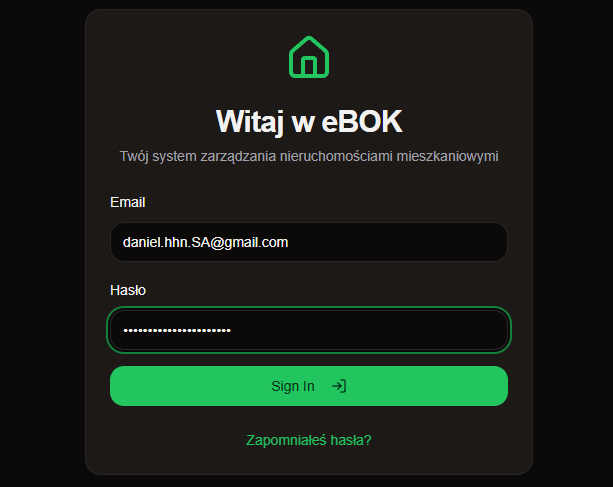
\includegraphics[scale=.6]{rys0C/logowanie_do_systemu}
		\caption{Logowanie do systemu jako super administrator}
	\label{fig:logowanie}
\end{figure}

\noindent \textbf{Dodanie nowego użytkownika do systemu~~}
Na panelu pracownika (rys.~\ref{fig:widoki}a), po lewej stronie widoczne są różne opcje do wyboru. Zawartość wyświetlana w części centralnej zależy wybranej opcji. W przypadku wybrania \texttt{Użytkownicy}, w części centralnej pojawi się zakładka zarządzania użytkownikami (rys.~\ref{fig:widoki}b), zaś w przypadku wybrania opcji \texttt{Mieszkania} -- zakładka do zarządzania mieszkaniami (rys.~\ref{fig:widoki}c).
Dodawanie nowego użytkownika można zrealizować na zakładce zarządzania użytkownikami. Wystarczy kliknąć na zielonym przycisku \texttt{Dodaj Użytkownika}. W reakcji na to kliknięcie otworzy się formularz, na którym można wprowadzić dane użytkownika, takie jak imię, nazwisko, e-mail, numer telefonu, hasło oraz rolę (rys.~\ref{fig:widoki}d). W omawianym przypadku należy wybrać rolę \texttt{ROLE\_OWNER}, co jest potrzebne by wykonać kolejny krok.
\begin{figure}[htb]
	\centering
  \begin{tabular}{@{}l@{}}
		a) \\  \vtop{\vskip-2ex\hbox{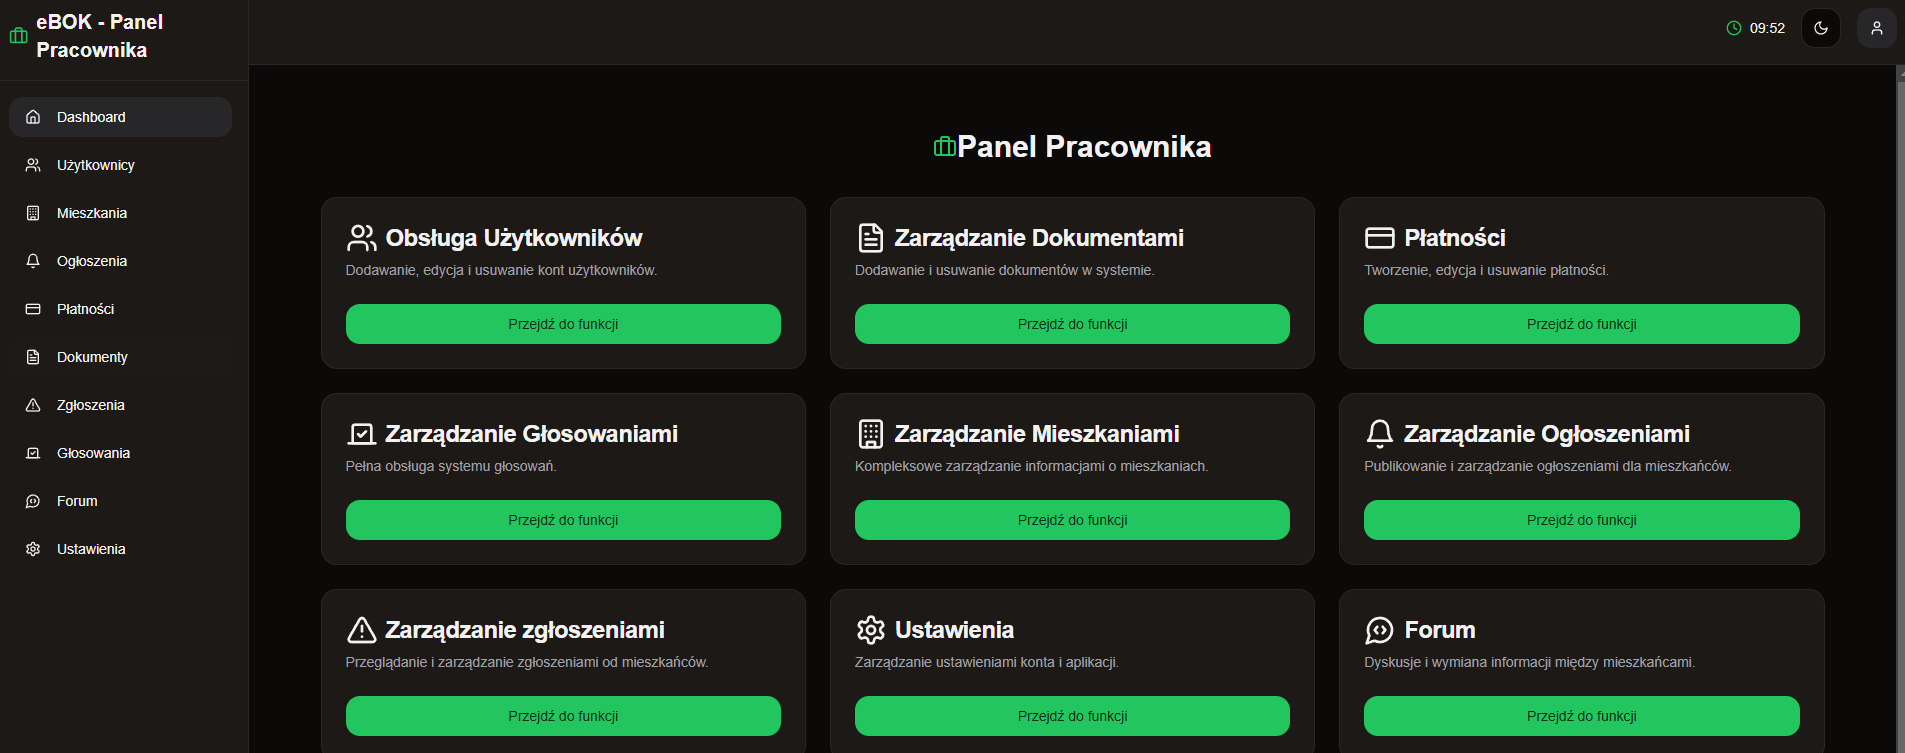
\includegraphics[width=\linewidth]{rys0C/panel_glowny_pracownika}}}\\
		b) \\  \vtop{\vskip-2ex\hbox{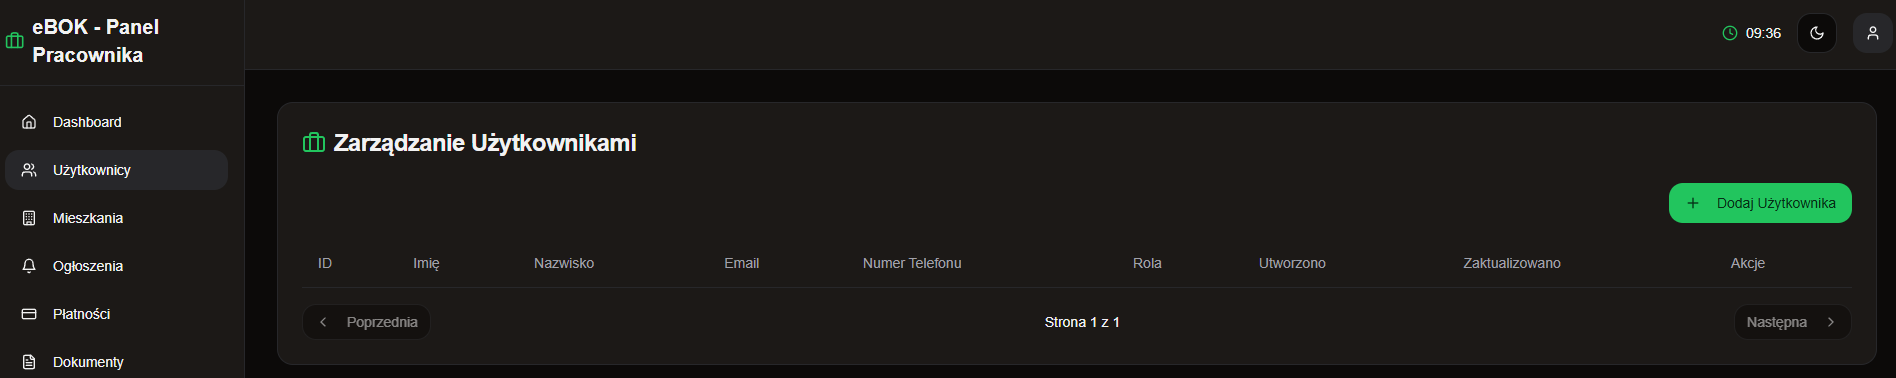
\includegraphics[width=\linewidth]{rys0C/zoskladka_do_uzytkownikow}}}\\
		c) \\ \vtop{\vskip-2ex\hbox{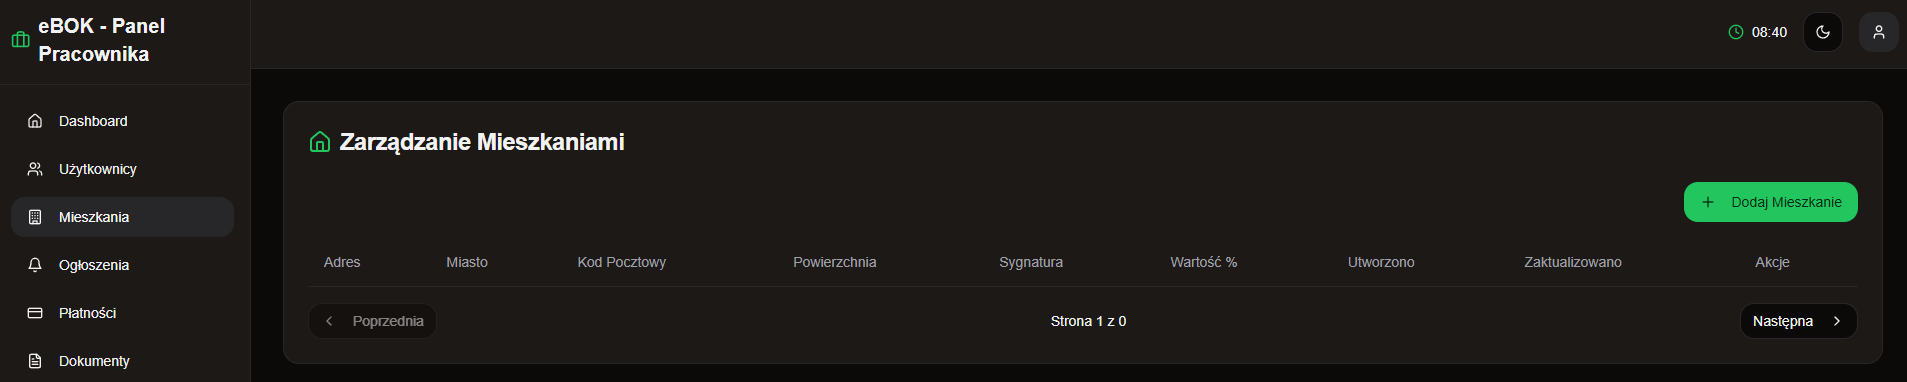
\includegraphics[width=\linewidth]{rys0C/zakladka_od_mieszkan}}} \\
		{\begin{tabularx}{\linewidth}{@{}XX@{}}
		d) &   e) \\
		\vtop{\vskip-2ex\hbox{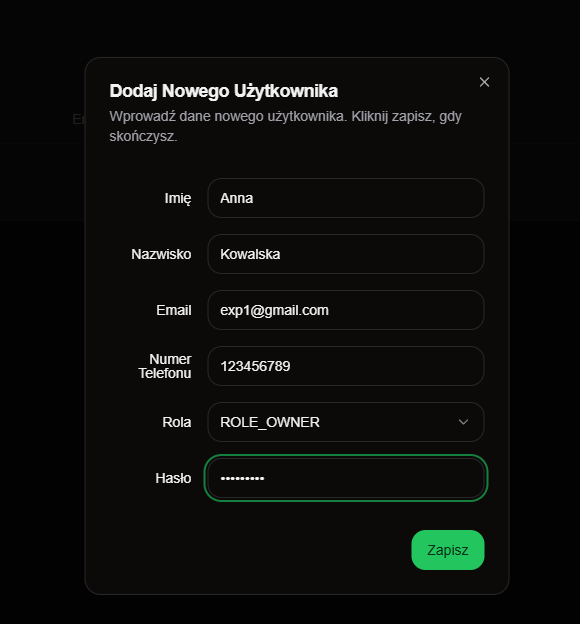
\includegraphics[scale=.6]{rys0C/dodanie_wlasciela}}} &
		\vtop{\vskip-2ex\hbox{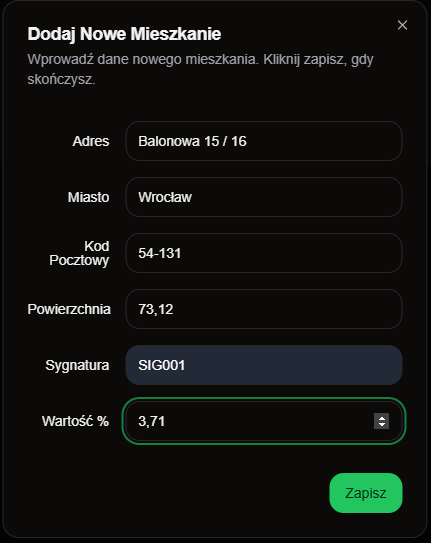
\includegraphics[scale=.6]{rys0C/dodanie_nowego_mieszkania}}}
		\end{tabularx}}
  \end{tabular}
		\caption{Widoki aplikacji: a) panel główny pracownika, b) zakładka zarządzania użytkownikami, c) zakładka zarządzania mieszkaniami}
	\label{fig:widoki}
\end{figure}
\clearpage

%\begin{figure}[htb]
    %\centering
    %\begin{tabular}{ll}
		%a) &   b) \\
		%\vtop{\vskip-2ex\hbox{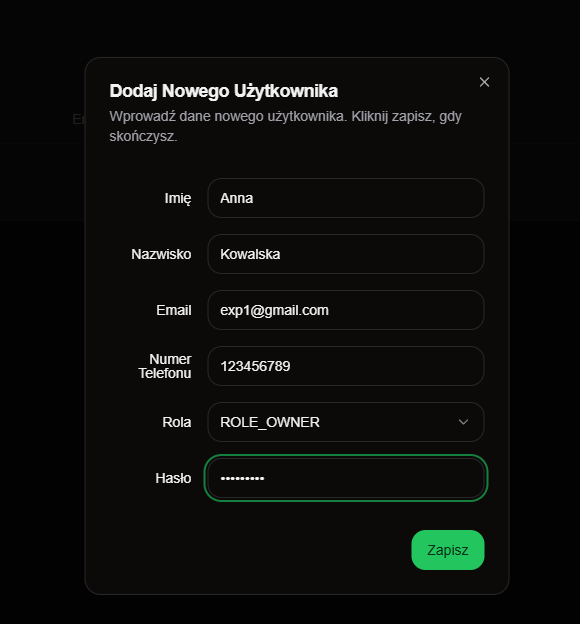
\includegraphics[scale=.6]{rys0C/dodanie_wlasciela}}} &
		%\vtop{\vskip-2ex\hbox{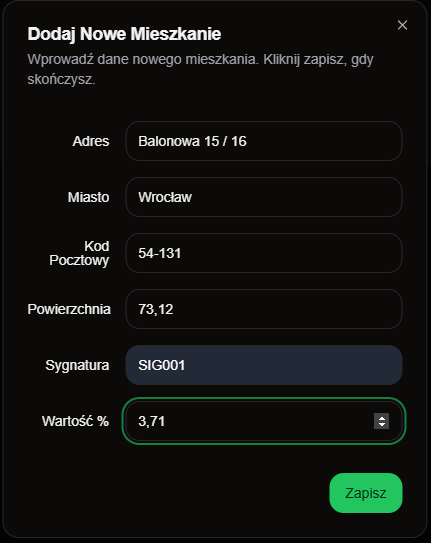
\includegraphics[scale=.6]{rys0C/dodanie_nowego_mieszkania}}}
		%\end{tabular}
    %\caption{Formularze dodawania: a) nowego użytkownika, b) nowego mieszkania}
    %\label{fig:add}
%\end{figure}


\noindent \textbf{Dodanie nowego mieszkania do systemu~~}
Aby dodać nowe mieszkanie, należy przejść do wspomnianej zakładki \texttt{Mieszkania}. Po tej czynności w części centralnej pojawi się Panel zarządzania mieszkaniami (rys.~\ref{fig:widoki}c). Kliknięcie na zielonym przycisku \texttt{Dodaj Mieszkanie} występującym na tej zakładce spowoduje wyświetlenie  formularza dodawania mieszkania (rys.~\ref{fig:widoki}e). W formularzu należy uzupełnić takie dane, jak adres, miasto, kod pocztowy, powierzchnia, sygnatura oraz procent udziału w nieruchomości.

\noindent \textbf{Przypisanie użytkownika do mieszkania~~} Po zakończeniu procesu dodawania nowego mieszkania zostanie ono uwidocznione na liście jak pokazano na rysunku~\ref{fig:apartment}a. Bezpośrednio po dodaniu mieszkanie nie będzie miało przypisanych właścicieli.
Aby tę sytuację zmienić należy przypisać właściciela do mieszkania. W tym celu należy na zarządzania mieszkaniami (rys.~\ref{fig:apartment}a) wybrać opcję \texttt{Przypisz Użytkownika} dostępną w kolumnie \texttt{Akcje}. Po wybraniu tej opcji otworzy się okienko (rys.~\ref{fig:apartment}b), w którym należy podać identyfikator użytkownika (\texttt{ID}) (to miejsce na identyfikator użytkownika dodanego wcześniej do systemu jako właściciel). Po pomyślnym przypisaniu właściciela system wyświetla zaktualizowaną listę właścicieli, jak przedstawiono na rysunku~\ref{fig:apartment}c.

\begin{figure}[htb]
    \centering
    \begin{tabular}{@{}l@{}}
		a) \\  \vtop{\vskip-2ex\hbox{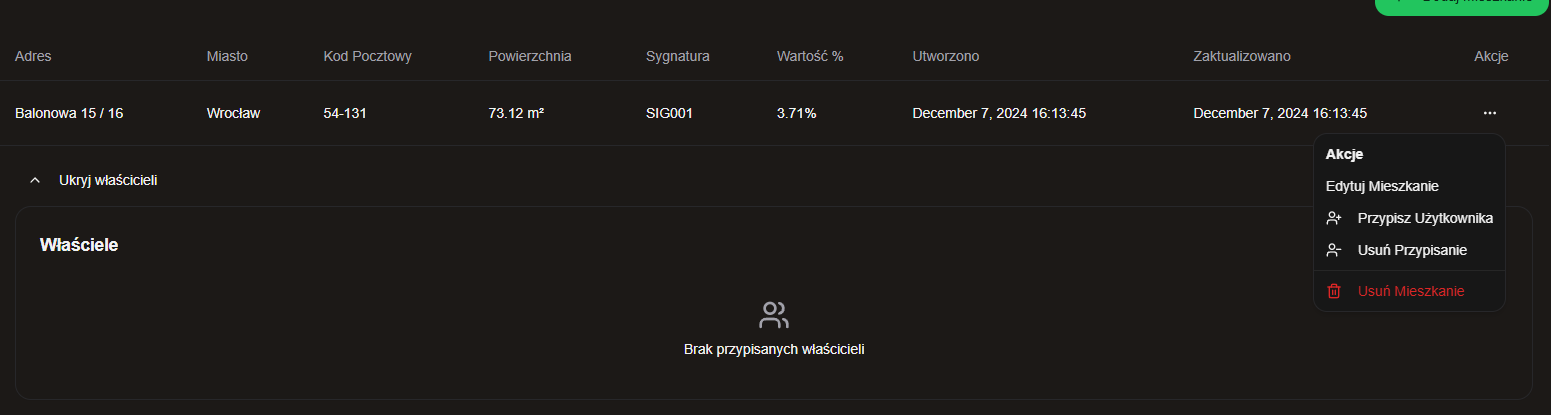
\includegraphics[width=\linewidth]{rys0C/jak_dodac_wlasciciela_1}}} \\
		b) \\  \vtop{\vskip-2ex\hbox{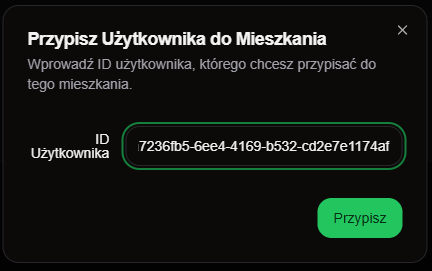
\includegraphics[scale=.55]{rys0C/jak_dodac_wlasciciela_2}}} \\
    c) \\  \vtop{\vskip-2ex\hbox{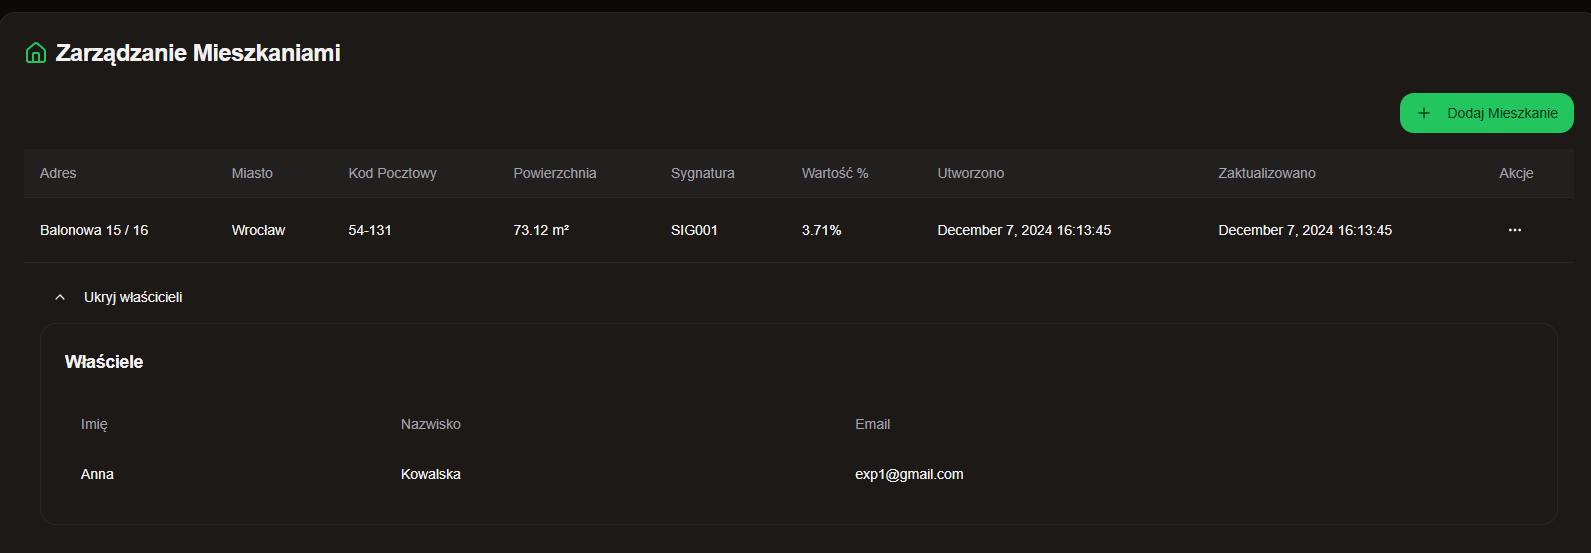
\includegraphics[width=\linewidth]{rys0C/wlasciciel_dodany}}}
		\end{tabular}
    \caption{Dodawanie nowego mieszkania: a) dane nowego mieszkania bez przypisanego właściciela, b) przypisywania właściciela do mieszkania, c) wynik udanego przypisanie właściciela do mieszkania}
    \label{fig:apartment}
\end{figure}



% LITERATURA (zostanie wygenerowana automatycznie)
%UWAGA: bibliotekę referencji należy przygotować samemu. Dobrym do tego narzędziem jest JabRef.
%       JabRef oferuje jednak większą liczbę typów rekordów niż obsługuje BibTeX.
%       Proszę nie deklarować rekordów o typach nieobsługiwanych przez BibTeX.
%       Formatowania wykazu literatury i cytowań odbywać się ma zgodnie z zadeklarowanym stylem.
%       Zalecane są style produkujące numeryczne cytowania (w postaci [1], [2,3]).
%       Takim stylem jest np. plabbrv
\bibliographystyle{plabbrv}
%       Aby zapanować nad odstępami w wykazie literatury można posłużyć się poniższą komendą
\setlength{\bibitemsep}{2pt} % - zacieśnia wykaz
%       Pozycja Literatura pojawia się w spisie treści nieco inaczej niż spisy rysunków, tabel itp.
%       Aby zachować właściwe odstępy należy użyć poniższej komendy
\addtocontents{toc}{\addvspace{2pt}} % ustawiamy odstęp w spisie treści przed pozycją Literatura 
%       Nazwę pliku przygotowanej biblioteki wpisuje się bez rozszerzenia .bib
%       (linia poniżej załaduje rekordy z pliku "dokumentacja.bib")
\bibliography{dokumentacja}


% Jeśli w pracy pojawiać się ma indeks, należy odkomentować poniższe linie
%%\chapterstyle{noNumbered}
%%\phantomsection % sets an anchor
%%\addcontentsline{toc}{chapter}{Indeks rzeczowy}
%%\printindex

\end{document}
